\section{Meccanica Lagrangiana}


\subsection{Sistemi potenziali newtoniani}

Consideriamo il sistema newtoniano costruito da $n $ particelle di masse $m_1,m_2,\dots,m_n$, interagenti tramite forze potenziali.\\
Precisamente supponiamo esista un potenziale:
\begin{equation}
    U(x^{(1)}, \dots, x^{(n )},t) \quad \text{ con } x^{(i )}\in \mathbb{R}^d  
\end{equation}
dove $x^{(i )}$ è la posizione della $i $-esima particella.\\
Tale che:
\begin{equation}
    f^{(i)}:= -\nabla_{(x^{(i)})}U= -\pdv{U}{x^{(i)}}= -\begin{pmatrix}
        \partial_{x^{(i)}_1}U\\
        \vdots\\
        \partial_{x^{(i)}_d}U
    \end{pmatrix}
\end{equation}
Il sistema di equazioni di Newton diventa:
\begin{equation}
    m_i\ddot{x}^{(i)}= f^{(i)}= -\pdv{U}{x^{(i)}}\iff\begin{cases}
        m_1\ddot{x}^{(1)}= \pdv{U}{x^{(1)}}\\
        \vdots\\
        m_n \ddot{x}^{(n)}= \pdv{U}{x^{(n)}}
    \end{cases}
\end{equation}
\begin{theorem}
    \begin{equation*}
        \pdv{U}{t}=0\implies H = \sum_{i=1}^{n}\frac{m_i}{2}\abs{\dot{x}^{(i)}}^2 + U (x^{(1)},\dots,x^{(n)}) \text{  si conserva.}
    \end{equation*}
\end{theorem}
\begin{proof}
    \begin{equation*}
        \dv{H}{t}= \sum_{i=1}^{n} m_i \dot{x}^{(i)}\cdot\ddot{x}^{(i)}+ \sum_{i=1}^{n}\pdv{U}{x^{(i)}}\cdot \dot{x}^{(i)}
    \end{equation*}
    \begin{equation*}
        = \sum_{i=1}^{n} \dot{x}^{(i)}\left( m_i\ddot{x}^{(i)}+\pdv{U}{x^{(i)}} \right)=0
    \end{equation*}
\end{proof}

Per comodità definifiamo:
\begin{equation}
    X:=\begin{pmatrix}
        x^{(1)}\\\vdots\\x^{(n )}
    \end{pmatrix}
    \in \mathbb{R}^d \times \dots \times \mathbb{R}^d \simeq \mathbb{R}^{nd}\qquad N = nd
\end{equation}
\begin{equation}
    \implies M\ddot{X}= -\nabla_X U\,; \qquad f = -\nabla_X U = \left( \pdv{U}{x^{(1)}};\dots;\pdv{U}{x^{(n)}} \right)\in \mathbb{R}^N 
\end{equation}
Dove la \textit{matrice delle masse }$M = \operatorname{diag} (m_1 \mathds{1}_d, \dots, m_n\mathds{1}_d)$ .
\begin{equation}
     M\ddot{X}= -\pdv{U}{X}\iff
    \begin{cases}
        \dot{X}= V\\\dot{V}= - M^{-1}\nabla_X U
    \end{cases}
\end{equation}
$X \in \mathbb{R}^N$ si dice \textit{spazio delle configurazioni del sistema}.\\
$(X,V)\in \mathbb{R}^N \times \mathbb{R}^N \simeq \mathbb{R}^{2N}$ si dice \textit{spazio delle fasi del sistema}.

\begin{samepage}
Affronteremo due problemi:
\begin{itemize}
    \item Come studiare il sistema in casi di dinamica vincolata:\begin{equation*}
        \begin{cases}
            M\ddot{X}= -\nabla_X U\\ X \in \mathcal{M}
        \end{cases}
        \end{equation*}
        dove $\mathcal{M}$ è una varietà differenziabile.
    \item Come varia il sistema sottoposto a un cambio di coordinate:\begin{equation*}
        \begin{cases}
            M\ddot{X} = -\nabla_X U\\ X \rightarrow X'
        \end{cases}
    \end{equation*}
\end{itemize}
\end{samepage}

\paragraph{Vincoli}
Esistono diversi tipi di vincoli:
\begin{itemize}
    \item \textbf{Vincolo bilatero:} vincola la particella a muoversi su una determinata curva o superficie.
    \item \textbf{Vincolo unilatero: } vincola la particella a non attraversare il determinato vincolo.
\end{itemize}
Noi ci limiteremo a studiare i vincoli bilateri e posizionali (\textit{olonomi}), che coinvolgono solo la posizione e non le velocità.

\begin{example}
    \textbf{Cerchio di raggio $r$}
    \begin{equation*}
        f(x_1,x_2)= x_1^2+x_2^2-r=0
    \end{equation*}
\end{example}

%fare meglio esempio e aggiunugere sfera e paraboloide


\subsection{Varietà differenziali}

\begin{definition}
    Data una funzione $\Phi: \mathbb{R}^N \times \mathbb{R}\rightarrow \mathbb{R}^M:(X,t)\mapsto \Phi(X,t)$ di classe $\mathcal{C}^1$,
    l'insieme di livello $\Phi^{-1}(0)= \left\{ X\in \mathbb{R}^N \;t.c.\; \Phi(x,t)=0\right\}$ definisce una \textit{varietà differenziabile}
    di classe $\mathcal{C}^1$ e dimensione $L=N-M $ se 
    \begin{equation}
        \pdv{\Phi}{X}= \pdv{\left( \Phi_1,\dots,\Phi_M \right)}{\left( X_1,\dots, X_N \right)}
    \end{equation} ha rango massimo $M $.
\end{definition}
\begin{theorem}
    Data $\Phi^{-1}(0) $ varietà differenziabile, esiste sempre \textit{rappresentazione cartesiana locale} per almeno un set di $L $ cooridnate libere:
    \begin{equation}
        \begin{cases}
            X_1 = g_1(X_{M+1},\dots,X_N)\\\vdots\\X_M = g_M (X_{M+1},\dots, X_N )
        \end{cases}
    \end{equation}
    Inoltre esiste una \textit{rappresentazione parametrica}.
\end{theorem}
\begin{proof}
    La prima parte si dimostra con il teorema di Dini, la seconda è ovvia. Riscriviamo le \( X_{M+1}, \dots, X_N \) come funzione di parametri liberi (cambio di coordinate) \( X_{M+i} = h_i(n_1, \dots, n_L) \) (può bastare \( X_{M+i} = n_i \)), e poi:
    \begin{equation*}
        \begin{cases}
            X_1 = g_1(f_1(n), \dots, f_L(n), t) := h_1(n, t)\\
            \vdots\\
            X_M = g_M(f_1(n), \dots, f_L(n), t) := h_M(n, t)\\
            X_{M+1} = f_1(n) := h_{M+1}(n, t)\\
            \vdots\\
            X_N = f_L(n) := h_N(n, t)
        \end{cases}
    \end{equation*}
    In conclusione, possiamo pensare alla varietà \(\mathcal{M}_t\) come localmente definita in forma parametrica \( \mathbb{R}^L \ni \vec{n} \mapsto X(\vec{n}, t) \in \mathbb{R}^N \), con dipendenza esplicita dal tempo.
\end{proof}

\begin{definition}
    $M= N-L $ si dice \textit{codimensione} delle varietà, che è la dimensione dello spazio normale.
\end{definition}

\begin{example}
    \(\Phi: \mathbb{R}^3 \times \mathbb{R} \rightarrow \mathbb{R}^2\), con \(N = 3\), \(M = 2\), \(L = 1\).\\
    Deve valere:
    \begin{equation*}
        \begin{cases}
            \Phi_1(x_1,x_2,x_3,t) = 0\\
            \Phi_2(x_1,x_2,x_3,t) = 0
        \end{cases}
    \end{equation*}
    Allora lo $\operatorname{span} \,\langle \nabla \Phi_1, \nabla \Phi_2 \rangle $ è il piano normale alla curva.
\end{example}

\begin{remark}
    Una varietà differenziabile $\mathcal{M}$ di classe $\mathcal{C}^1$ ammette sempre una rappresentazione locale parametrica,
    \begin{equation*}
        u \in \mathbb{R}^L \mapsto X(u, t) \in \mathbb{R}^N
    \end{equation*}
    Le $L$ derivate parziali rispetto ai parametri, ottenute fissandone $L-1$ alla volta in un punto, generano $L$ curve differenziabili. Le loro derivate generano lo spazio tangente alla varietà, ovvero il piano tangente nel punto fissato.
\end{remark}

\begin{definition}
    Lo \textit{spazio tangente} a $\mathcal{M}$ nel punto $X^\ast = X(u_1^\ast,\dots, u_L^\ast)$ è:
    \begin{equation*}
        T_X \mathcal{M} = \operatorname{span} \left\{ \pdv{X(u_1^\ast, u_L^\ast)}{u_1},\dots, \pdv{X(u_1^\ast,\dots, u_L^\ast)}{u_L} \right\}
    \end{equation*}
\end{definition}

\begin{definition}
    Lo \textit{spazio ortogonale} a $T_X \mathcal{M}$ si dice $N_X \mathcal{M}$:
    \begin{equation*}
        N_X \mathcal{M} = \operatorname{span} \left\{ \nabla_X \Phi_1,\dots, \nabla_X \Phi_M  \right\}
    \end{equation*}
\end{definition}

\begin{remark}
    Vale la decomposizione $T_X \mathcal{M} \oplus N_X \mathcal{M} = \mathbb{R}^N$
\end{remark}

\begin{remark}
    $\Phi_i(X(u)) \equiv 0 \quad \text{per } i = 1, \dots, M$
\end{remark}

\begin{equation*}
    \pdv{\Phi_i(X(u))}{u_s} = \sum_{k=1}^N \pdv{\Phi_i}{X_k}\bigg|_{X(u)} \pdv{X_k}{u_s} = \pdv{\Phi_i}{X} \cdot \pdv{X}{u_s} = 0
\end{equation*}

\begin{equation*}
    \Rightarrow N_X \mathcal{M} \perp T_X \mathcal{M} \qquad 
    \pdv{X}{u_s} \cdot \left( \sum_{i=1}^M \pdv{\Phi_i}{X} \right) = 0
\end{equation*}


\subsection{Sistemi potenziali vincolati}

\begin{definition}
    Un \textit{sistema newtoniano potenziale} soggetto a vincoli olonomi bilateri ideali e (possibilmente) dipendenti dal tempo è definito da:
    \begin{equation*}
        M\ddot{X} = -\nabla_X U + R \qquad (X \in \mathbb{R}^N), \quad X(0) \in \mathcal{M}, \quad \dot{X}(0) \in T_{X(0)}\mathcal{M}
    \end{equation*}
    con $R \perp T_X \mathcal{M}$ per ogni $X \in \mathcal{M}$ (ossia $R \in N_X \mathcal{M}$).
\end{definition}

Noi useremo la rappresentazione: $q \in \mathbb{R}^L \mapsto X(q, t) \in \mathbb{R}^N$, 
il caso $L= N$ è un semplice cambio di coordinate dove è assunto $R =0$.
\begin{theorem}
    \textbf{Lagrange}\\
    La dinamica di un sistema newtoniano potenziale in $\mathcal{M}$, come appena definito, è determinato dalle \textit{equazioni di Lagrange}:
    \begin{equation}
        \dv{}{t}\left( \pdv{\mathcal{L}}{\dot{q}_i} \right)-\pdv{\mathcal{L}}{q_i}=0 \qquad i = 1,\dots, L 
    \end{equation}
    in cui $\mathcal{L}:= \eval{K-U}_{\mathcal{M}};\quad \mathcal{L}(q,\dot{q},t)$ è detta \textit{lagrangiana}. \\
    La reazione è data da $R = M\ddot{X}+\eval{\nabla_X U }_{\mathcal{M}}$.
\end{theorem}
\begin{remark}
    Il moto su $\mathcal{M}$ è descritto da $t\mapsto q(t)$, soluzione delle equazioni di Lagrange.
\end{remark}
\begin{proof}
    Proiettiamo $M\ddot{X} = -\nabla_X U + R$ in $T_X\mathcal{M}$:
    \begin{equation*}
        M\ddot{X}\cdot \pdv{X}{q_i}= -\nabla_X U \cdot \pdv{X}{q_i}+ R\cdot\pdv{X}{q_i}= -\nabla_X U \cdot \pdv{X}{q_i}
        = -\pdv{U}{q_i}\left( x(q,t),t   \right)= \eval{ -\pdv{U}{q_i}}_{\mathcal{M}}
    \end{equation*}
    \begin{equation}
        M\ddot{X}\cdot \pdv{X}{q_i}= \dv{}{t}\left( M\dot{X}\cdot \pdv{X}{q_i} \right)-M\dot{X}\cdot\dv{}{t}\pdv{X}{q_i}
    \end{equation}
    Utilizziamo due lemmi da dimostrare successivamente:
    \begin{equation}
        1) \; \pdv{\dot{X}_k}{\dot{q}_i}= \pdv{X_k}{q_i} \qquad 2)\; \dv{}{t}\pdv{X_k}{q_i}= \pdv{\dot{X}_k}{q_i}\qquad k = 1,\dots,N;\; i = \, 1,\dots, L 
    \end{equation}
    Quindi otteniamo:
    \begin{equation*}
        = \dv{}{t}\left( M\dot{X}\cdot\pdv{\dot{X}}{\dot{q}_i} \right)-M\dot{X}\cdot \pdv{\dot{X}}{q_i}
    \end{equation*}
    Consideriamo poi:
    \begin{equation*}
        \pdv{}{\dot{q}_i}\left( M\dot{X}\cdot\dot{X} \right)= M\pdv{\dot{X}}{\dot{q}_i}\cdot\dot{X}+ M\dot{X}\cdot\pdv{\dot{X}}{\dot{q}_i}=
        \pdv{\dot{X}}{\dot{q}_i}\cdot M^\intercal \dot{X} + M\dot{X}\cdot\pdv{\dot{X}}{\dot{q}_i}= 2\left( M\dot{X}\cdot\pdv{\dot{X}}{\dot{q}_i} \right)
    \end{equation*}
    Dove nell'ultimo passaggio abbiamo utilizzato $M^\intercal= M$ perché simmetrica. Utilizzando questo otteniamo:
    \begin{equation*}
        M\ddot{X}\cdot\pdv{X}{q_i}= \dv{}{t}\left( \pdv{}{\dot{q}_i }\left( \frac{1}{2}M\dot{X}\cdot\dot{X} \right) \right)- \pdv{}{q_i}\left( \frac{1}{2}M\dot{X}\cdot\dot{X} \right)
    \end{equation*}
    Ricordando che $\frac{1}{2}M\dot{X}\cdot\dot{X}= K$ energia cinetica del sistema e eguagliando alla prima equazione:
    \begin{equation*}
        \dv{}{t} \left( \pdv{\dot{q}_i} \eval{K}_{\mathcal{M}} \right)- \pdv{}{q_i}\eval{K}_{\mathcal{M}}= -\pdv{}{q_i} \eval{U}_{\mathcal{M}} \;;\qquad \pdv{U}{\dot{q}_i}=0
    \end{equation*}
    \begin{equation}
        \dv{}{t}\left( \pdv{}{\dot{q}_i} \eval{K-U}_{\mathcal{M}} \right)-\pdv{}{q_i}\eval{K-U}_{\mathcal{M}}
    \end{equation}
    Nel caso non vincolato: $R = 0, L = N$.
\end{proof}

\begin{remark}
    La dimostrazione non fa uso specifico della parametrizzazione, perciò le equazioni di Lagrange sono invarianti in forma:
    \begin{equation}
        q = q(\tilde{q})\implies \tilde{X}(\tilde{q},t)\equiv X ( q(\tilde{q}),t)
    \end{equation}
\end{remark}
\begin{proof}
    Dimostriamo ora i due lemmi che abbiamo usato precedentemente:
    \begin{equation}
        1)\;\pdv{X_k}{q_i}= \pdv{\dot{X}_k}{\dot{q}_i}: \quad \dot{X}= \dv{X_k}{t}(q(t),t)= \sum_{l=1}^{L}\pdv{X_k}{q_l}\dot{q}_l+ \pdv{X_k}{t}\implies\pdv{\dot{X}_k}{\dot{q}_i}= \pdv{X_k}{q_i}
    \end{equation}
    \begin{equation}
        2)\;\dv{}{t}\pdv{X_k}{q_i}: \quad \pdv{\dot{X}_k}{q_i}= \sum_{j=1}^{L}\pdv{X_k}{q_i}{q_j}\dot{q}_j+\pdv{X_k}{q_i}{t}
        \qquad \dv{}{t}\pdv{X_k}{q_i}= \sum_{j= 1}^{L }\pdv{X_k}{q_j}{q_i}\dot{q}_j +\pdv{X_k}{t}{q_i}
    \end{equation}
    che sono uguali se vale Schwartz, cioé quando sono $\mathcal{C}^2$.
\end{proof}

\begin{example}
    \textbf{Pendolo}\\
    Vincolato a una varietà differenziale $\mathcal{M}$ a forma circolare di raggio $l$. Scriviamo la lagrangiana:
    \begin{equation}
        \eval{\mathcal{L}}_{\mathcal{M}}= \eval{K-U}_{\mathcal{M}}= \frac{m}{2}\abs{\dot{x}}^2-mg x_2= 
        \frac{ml^2\dot{\theta}^2}{2}+ mgl\cos(\theta)
    \end{equation}
    \begin{equation}
        \dv{t}\pdv{\mathcal{L}}{\dot{\theta}}-\pdv{\mathcal{L}}{\theta}= ml^2\ddot{\theta}+mgl\sin(\theta)= 0 
    \end{equation}
\end{example}

\begin{example}
    \textbf{Moto potenziale conservativo centrale}\\
    In generale per una particella sottoposta a un potenziale $U(r )$ con $r = \abs{x}$:
    \begin{equation}
        \mathcal{L}= \frac{m}{2}\abs{\dot{x}}^2 -U(\abs{x}) = \frac{m}{2}\left( \dot{r}^2+r^2\dot{\theta}^2 \right)-U(r)
    \end{equation}
    \begin{equation}
        \dv{t}\pdv{\mathcal{L}}{\dot{r}}-\pdv{\mathcal{L}}{r}= \dv{t}\left( m\dot{r} \right) - mr\dot{\theta}^2 + \pdv{U}{r}=0\qquad 
        \dv{t}\pdv{\mathcal{L}}{\dot{\theta}}-\pdv{\mathcal{L}}{\theta}= \dv{t}\left( mr^2\dot{\theta} \right)=0
    \end{equation}
    \begin{equation}
        \begin{cases}
            m\ddot{r}= r\dot{\theta}^2-\pdv{U}{r}= \frac{\ell^2}{mr^3}-U'(r)= -\dv{r}\left( U(r) + \frac{\ell^2}{2mr^2} \right)\\
            mr^2\dot{\theta}= \text{ costante }= \ell
        \end{cases}
    \end{equation}
\end{example}

\begin{definition}
    Le coordinate che non appaiono in $\mathcal{L}$, cioè $\pdv{\mathcal{L}}{q_i}=0$, si dicono \textit{cicliche} o \textit{ignorabili}.
\end{definition}
\begin{proposition}
    Se $q_i $ è coordinata ciclica, il \textit{momento associato a }$q_i $ $p_i:=\pdv{\mathcal{L}}{\dot{q}_i}$ è costante del moto.
\end{proposition}
\begin{remark}
    $p_i$ è funzione di $q,\dot{q}$ e $t$.
\end{remark}
\begin{remark}
    Simmetrie generano coordinate cicliche (teorema di Noether).
\end{remark}

\begin{example}
    Se per i moti centrali teniamo le coordinate cartesiane, non si hanno cicliche.
\end{example}

Consideriamo ora come scrivere il quadrato delle velocità in diversi sistemi di coordinate:
\begin{itemize}
    \item \textbf{Cartesiane}: $\dd{s^2}= \dd{x}\cdot\dd{x}= \dd{x_1^2}+\dd{x_2^2}+\dd{x_3^2}\implies v^2= \dot{x}_1^2+\dot{x}_2^2+\dot{x}_3^2$
    \item \textbf{Polari piane}: $\dd{s^2}= \dd{r^2}+r^2\dd{\theta^2}\implies v^2=\dot{r}^2+r^2\dot{\theta}^2$
    \item \textbf{Cilindriche}: $\dd{s^2}= \dd{r^2}+r^2\dd{\theta^2}+\dd{z^2}\implies v^2= \dot{r}^2+r^2\dot{\theta}^2+\dot{z}^2$
    \item \textbf{Polari sferiche}: $\dd{s^2}= \dd{r^2}+r^2\dd{\theta^2}+r^2\sin[2](\theta)\dd{\varphi^2}\implies v^2 = \dot{r}^2+r^2\dot{\theta}^2+r^2\sin[2](\theta)\dot{\varphi}^2$
\end{itemize}


\subsection{Energia}

\begin{definition}
    La dimensione della varietà differenziale $\mathcal{M}$ si dice \textit{numero di gradi di libertà} $L$. Lo spazio della fasi avrà dimensione $2L$.
\end{definition}
Per sistemi non vincolati di $n $ particelle in $\mathbb{R}^d$: $L = N = nd$.

\begin{remark}
    $\dot{X}= \pdv{X}{q}\cdot \dot{q}+ \pdv{X}{t}$ possiamo dunque scrivere l'energia cinetica come:
    \begin{equation}
        \eval{K}_{\mathcal{M}}= \left( \pdv{X}{q}\cdot \dot{q}+ \pdv{X}{t} \right)\cdot \frac{M}{2}\left( \pdv{X}{q}\cdot \dot{q}+ \pdv{X}{t} \right)= K_2+K_1+K_0
    \end{equation}
    Dove consideriamo:
    \begin{align}
    K_2 &= \left( \pdv{X}{q}\cdot \dot{q} \right)\cdot \frac{M}{2}\left( \pdv{X}{q}\cdot \dot{q} \right)= \frac{1}{2}\dot{q}\cdot A(q,t)\dot{q}\\
    K_1 &= \left( \pdv{X}{q}\cdot \dot{q} \right)\cdot M\pdv{X}{t}=B(q,t)\cdot \dot{q}\\
    K_0 &= \frac{1}{2}\pdv{X}{t}\cdot M\pdv{X}{t}= C (q,t) 
    \end{align}
    dove $A$ è una matrice $L\times L $, $B $ è un vettore di dimensione $L $ e $C $ è uno scalare.
\end{remark}

\begin{remark}
    $A(q,t)$ è una matrice simmetrica definita positiva.
\end{remark}
\begin{proof}
    \begin{equation*}
        K_2 = \frac{1}{2}\left( \dot{q} \cdot \pdv{X}{q} \right) \cdot M \left( \pdv{X}{q} \cdot \dot{q} \right)
        = \frac{1}{2} \sum_{k,m=1}^{N} \sum_{i,j=1}^{L} \dot{q}_i \pdv{X_k}{q_i} M_k \delta_{km} \pdv{X_m}{q_j} \dot{q}_j
    \end{equation*}
    \begin{equation}
        = \frac{1}{2} \sum_{i,j=1}^{L} \dot{q}_i \left( \sum_{k=1}^{N} \pdv{X_k}{q_i} \pdv{X_k}{q_j} M_k \right) \dot{q}_j
        \implies A_{ij}(q,t) = \sum_k \pdv{X_k}{q_i} \pdv{X_k}{q_j} M_k
    \end{equation}
    Che è un prodotto scalare e $M$ è positiva, quindi $A$ è simmetrica e positiva.
\end{proof}

Da quest'espressione di $K$ possiamo ricavare:
\begin{equation}
    K = K_2 + K_1 + K_0 = \frac{1}{2} \dot{q} \cdot A \dot{q} + B \cdot \dot{q} + C
    \implies \pdv{\mathcal{L}}{\dot{q}} = A \dot{q} + B
\end{equation}
\begin{equation}
    \implies \dv{t}(A \dot{q} + B) - \pdv{}{q} \left( \frac{1}{2} \dot{q} \cdot A \dot{q} + B \cdot \dot{q} + C - U \right) = 0
\end{equation}
\begin{equation*}
    \left( \pdv{A}{q} \dot{q} \cdot \dot{q} + \pdv{A}{t} \dot{q} + \pdv{B}{q} \dot{q} + \pdv{B}{t} \right)
    + A \ddot{q} - \pdv{}{q} \left( \frac{1}{2} \dot{q} \cdot A \dot{q} + B \cdot \dot{q} + C - U \right) = 0
\end{equation*}
\begin{equation}
    \implies A \ddot{q} + \left[ \dot{q} \right]_2 - \left[ \dot{q} \right]_2' = 0
    \implies A \ddot{q} = F(q, \dot{q}, t), \text{ di grado max } 2
\end{equation}
$A$ è definita positiva, $\implies \exists\,A^{-1}$:
\begin{equation}
    \ddot{q}= G(q,\dot{q},t):= A^{-1}F \iff 
    \begin{cases}
        \dot{q}= v\\\dot{v}= G(q,\dot{q},t)
    \end{cases}\implies \exists! \text{ locale}
\end{equation}

\begin{definition}
    Le $q_i $ si dicono \textit{coordinate generalizzate} e le $\dot{q}_i $ \textit{velocità generalizzate}.
\end{definition}
\begin{remark}
    $\dot{X}= \pdv{X}{q}\cdot \dot{q}+\pdv{X}{t}$ il termine $\pdv{X}{t}$ è legato allo spostamento della varietà.
\end{remark}

\begin{definition}
    \begin{equation}
        H(q,\dot{q},t):= p\cdot\dot{q}-\mathcal{L}= \pdv{\mathcal{L}}{\dot{q}}\cdot\dot{q}-\mathcal{L}
    \end{equation}
    si dice \textit{funzione energia} del sistema lagrangiano.
\end{definition}
\begin{proposition}
    $\dot{H}= -\pdv{\mathcal{L}}{t}$; se $\mathcal{L}$ non dipende esplicitamente da $t$, allora $\dot{H}=0$.
\end{proposition}
\begin{proof}
    \begin{equation*}
        \dv{H}{t}= \dv{t}\left( p\cdot\dot{q} \right)-\dv{\mathcal{L}}{t}= 
        \dot{p}\cdot\dot{q}+p\cdot\ddot{q}-\pdv{\mathcal{L}}{q}\cdot \dot{q}-\pdv{\mathcal{L}}{\dot{q}}\cdot\ddot{q}-\pdv{\mathcal{L}}{t}
    \end{equation*}
    \begin{equation*}
        = \left( p-\pdv{\mathcal{L}}{\dot{q}} \right)\cdot \ddot{q}+\left( \dot{p}-\pdv{\mathcal{L}}{q} \right)\cdot \dot{q}-\pdv{\mathcal{L}}{t}= -\pdv{\mathcal{L}}{t}
    \end{equation*}
\end{proof}

Per i sistemi meccanici $K = \frac{1}{2}\dot{q}\cdot A\dot{q}+ B\cdot \dot{q}+ C $:
\begin{equation*}
    \mathcal{L}= K-U\,;\qquad p = \pdv{\mathcal{L}}{\dot{q}}= \pdv{K}{\dot{q}}= A\dot{q}+B 
\end{equation*}
\begin{equation*}
    H = p \cdot \dot{q} - \mathcal{L} = (A\dot{q} + B) \cdot \dot{q} - \left( \frac{1}{2} \dot{q} \cdot A \dot{q} + B \cdot \dot{q} + C - U \right)
\end{equation*}
\begin{equation*}
    = \dot{q} \cdot A \dot{q} + B \cdot \dot{q} - \frac{1}{2} \dot{q} \cdot A \dot{q} - B \cdot \dot{q} - C + U
\end{equation*}
\begin{equation}
    = \frac{1}{2} \dot{q} \cdot A \dot{q} + U - C \equiv K_2 + U_{\text{EFF}} \qquad U_{\text{EFF}} := U - C
\end{equation}

\begin{example}
    \textbf{Pendolo in rotazione}

    \begin{figure}[h]
        \centering
        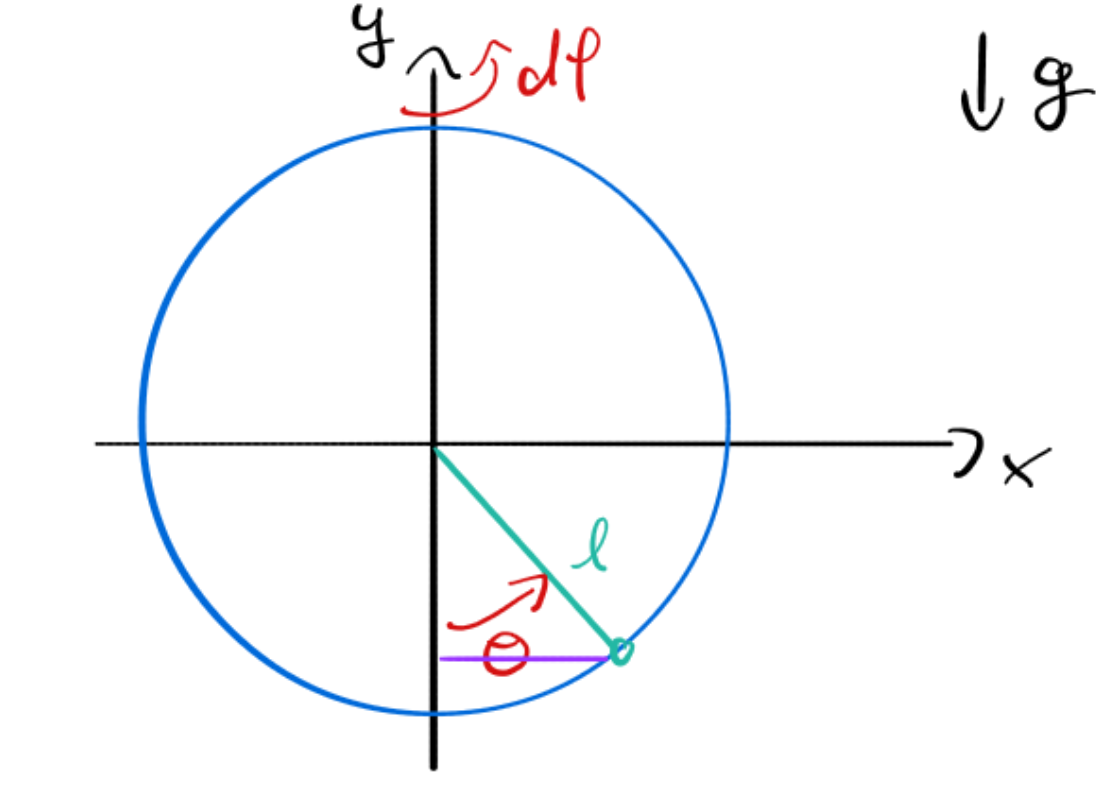
\includegraphics[width=0.6\textwidth]{images/pendoloInRotazione.png}
        \caption{Rappresentazione pendolo in rotazione}
    \end{figure}

    \begin{equation*}
        \dd{s}^2 = \ell^2 \dd{\theta}^2 + \ell^2 \sin^2\theta \, \omega^2 \dd{t}^2
        \implies K = \frac{1}{2}m \left( \ell^2 \dot{\theta}^2 + \ell^2 \sin^2\theta \, \omega^2 \right)
        \qquad U = mg(-\ell\cos\theta)
    \end{equation*}
    \begin{equation}
        \mathcal{L} = \frac{1}{2} m \ell^2 \dot{\theta}^2 + \frac{1}{2} m \ell^2 \sin^2\theta \, \omega^2 + mg\ell\cos\theta
    \end{equation}

    $\mathcal{L}$ non dipende esplicitamente dal tempo, perciò si conserva:
    \begin{equation}
        H = \pdv{\mathcal{L}}{\dot{q}}\dot{q}-\mathcal{L} =K_2-K_0+U
    \end{equation}
    \begin{equation*}
        H = m\ell^2 \dot{\theta} \cdot \dot{\theta} - \frac{m\ell^2}{2} \dot{\theta}^2 - \frac{m\ell^2}{2} \sin^2\theta \, \omega^2 - mg\ell \cos\theta
        = \frac{m\ell^2}{2} \dot{\theta}^2 - mg\ell \cos\theta - \frac{m\ell^2}{2} \omega^2 \sin^2\theta
    \end{equation*}
    \begin{equation}
        \implies \mathcal{L} = m\ell^2 \left[ \frac{\dot{\theta}^2}{2} + \frac{\omega^2}{2} \sin^2\theta + \frac{g}{\ell} \cos\theta \right]
        := m\ell^2 \mathcal{L}' \qquad
        \omega_g := \sqrt{\frac{g}{\ell}}
    \end{equation}
    \begin{remark}
        Le equazioni di Lagrange sono lineari, posso usare $\mathcal{L}$ o $\mathcal{L}'= c\mathcal{L}$ con $c\neq0$ e avere le stesse equazioni finali.
    \end{remark}
    \begin{equation*}
        H' = \frac{\dot{\theta}^2}{2}- \frac{\omega^2}{2}\sin[2](\theta) - \omega_g^2\cos(\theta)\implies E = \frac{\dot{\theta}^2}{2}+U_e(\theta)
    \end{equation*}
    
    \paragraph{Proprietà del potenziale efficace}
    Il potenziale efficace $U_e(\theta)$ è pari: $U_e(\theta) = U_e(-\theta)$. La derivata prima è
    \[
    U_e'(\theta) = -\omega^2 \sin\theta \cos\theta + \omega_g^2 \sin\theta
    \]
    Gli zeri di $U_e'(\theta)$ sono dati da
    \[
    U_e'(\theta) = 0 \iff (\omega_g^2 - \omega^2 \cos\theta)\sin\theta = 0
    \]
    quindi per $\theta = 0, \pi$ e, se $\omega > \omega_g$, anche per $\cos\theta = \frac{\omega_g^2}{\omega^2}$, cioè esistono due soluzioni simmetriche $\theta_\pm \simeq \pm \arccos\left(\frac{\omega_g^2}{\omega^2}\right)$.

    \paragraph{Stabilità degli equilibri}
    La derivata seconda è
    \[
    U_e''(\theta) = \omega_g^2 \cos\theta - \omega^2 \cos(2\theta)
    \]
    Per $\theta = 0$: $U_e''(0) = \omega_g^2 - \omega^2$ (stabile se $\omega < \omega_g$, instabile se $\omega > \omega_g$).\\
    Per $\theta = \pi$: $U_e''(\pi) = -\omega_g^2 - \omega^2$ (sempre instabile).\\
    Per $\theta = \theta_\pm$: $U_e''(\theta_\pm) = -\frac{\omega_g^4}{\omega^2} + \omega^2$, che è positivo se $\omega > \omega_g$ (stabile).

    \paragraph{Comportamento per piccoli angoli}
    Per $\omega < \omega_g$, il comportamento è simile al pendolo classico. Per $\theta$ piccoli:
    \[
    U_e(\theta) \simeq -\omega_g^2\left(1 - \frac{\theta^2}{2} \right) - \frac{\omega^2}{2} \theta^2 + o(\theta^4)
    = \frac{\omega^2_g-\omega^2}{2}\theta^2 -\omega^2_g +o(\theta^4)
    \]

    \paragraph{Transizione di stabilità}
    Quando $\omega$ raggiunge $\omega_g$, si inverte la concavità del potenziale efficace.

    \paragraph{Tipi di moto per $\omega > \omega_g$}
    \begin{itemize}
        \item $E < U(\theta_\pm)$: nessun moto
        \item $E = U(\theta_\pm)$: due punti di equilibrio (centri)
        \item $E \in \left( U(\theta_\pm), U(0) \right)$: due moti oscillatori
        \item $E = U(0) = -\omega_g^2$: punto iperbolico, due traiettorie omoclini
        \item $E > U(0)$: comportamento come un pendolo con due moti rotatori
    \end{itemize}

    %Finire qua....

\end{example}


\begin{example}
    \textbf{Pendolo sferico}\\
    La particella si muove su un anello libero di ruotare:
    \begin{equation}
        \dd{s^2}=\ell^2\dd{\theta^2}+\ell^2\sin[2](\theta)\dd{\varphi^2}\,;\qquad 
        K = \frac{m\ell^2}{2}\left( \dot{\theta}^2+\sin[2](\theta)\dot{\varphi^2} \right)
    \end{equation}
    \begin{equation}
        \mathcal{L}= \frac{m\ell^2}{2}\left( \dot{\theta}^2+\sin[2](\theta)\dot{\varphi^2} \right)+mg\ell\cos(\theta)
    \end{equation}
    E se l'anello avesse massa? $\dd{m}= \rho\dd{s}=\rho\ell\dd{\theta'}$
    \begin{equation*}
        K_{\text{anello}} = 2 \int_0^{\pi} \frac{1}{2} \, \rho \, \ell \, \dd{\theta'} \, \ell^2 \sin^2\theta' \, \dot{\varphi}^2
        = \frac{2}{2} \, \dot{\varphi}^2 \, \ell^3 \, \rho \int_0^{\pi} \sin^2\theta' \, \dd{\theta'}
    \end{equation*}
    \begin{equation}
        = \ell^3 \dot{\varphi}^2 \rho \int_0^{\pi} \frac{1 - \cos 2\theta}{2} \, \dd{\theta}
        = \frac{\ell^3 \dot{\varphi}^2 \rho}{2} \left[ \theta - \frac{\sin 2\theta}{2} \right]_0^{\pi}
        = \frac{\ell^3 \dot{\varphi}^2 \rho}{2} \cdot \pi
    \end{equation}
    \begin{equation}
        M = \rho \cdot 2\pi\ell \implies K_\text{anello}= \frac{M \ell^2 \dot{\varphi}^2}{4}\qquad
        r = \frac{M}{2m} \qquad \omega_g = \sqrt{\frac{g}{\ell}}
    \end{equation}
    \begin{equation}
        \implies \mathcal{L}= K-U = m\ell^2\left( \frac{1}{2}\dot{\theta}^2 +\frac{1}{2}\sin[2](\theta)\dot{\varphi}^2+ \frac{r}{2}\dot{\varphi}^2+ \omega^2_g\cos(\theta)\right)
    \end{equation}
    \begin{equation}
        \pdv{\mathcal{L}}{\varphi}=0\implies P_\varphi= \frac{\mathcal{L}'}{\dot{\varphi}}= \left( \sin[2](\theta)+r \right)\dot{\varphi}\equiv c \text{ costante}
    \end{equation}

    Il segno di $c $ è quello di $\dot{\varphi}(0)$. Studiamo $c>0$:
    \begin{equation}
        \dot{\varphi}(t)=\frac{c}{\sin[2](\theta(t))+r}>0 \quad \forall\;t
    \end{equation}
    \begin{equation*}
        \pdv{\mathcal{L}'}{t} = 0 \implies H' = K' + U' = \frac{\dot{\theta}^2}{2} + \frac{\sin^2\theta}{2} \dot{\varphi}^2 + \frac{r}{2} \dot{\varphi}^2 - \omega_g^2 \cos\theta
    \end{equation*}
    \begin{equation*}
        = \frac{\dot{\theta}^2}{2} + \frac{\sin^2\theta}{2} \cdot \frac{c^2}{(\sin^2\theta + r)^2} + \frac{r}{2} \cdot \frac{c^2}{(\sin^2\theta + r)^2} - \omega_g^2 \cos\theta
    \end{equation*}
    \begin{equation}
        = \frac{\dot{\theta}^2}{2} + \frac{c^2}{2(\sin^2\theta + r)} - \omega_g^2 \cos\theta = E := \frac{\dot{\theta}^2}{2} + U_e(\theta)
    \end{equation}

    Studiamo ora le orbite del sistema:
    \begin{equation}
        U_e(\theta) = \frac{1}{2} \cdot \frac{c^2}{\sin^2\theta + r} - \omega_g^2 \cos\theta \implies 
        U_e(\theta) = U_e(-\theta)
    \end{equation}
    \begin{equation}
        U_e'(\theta) = \omega_g^2 \sin\theta - \frac{c^2}{(\sin^2\theta + r)^2} \cdot 2\sin\theta \cos\theta
    \end{equation}
    \begin{equation}
        \implies U_e' = 0 \iff \theta = 0, \pi \text{ e le soluzioni di }
        (\sin^2\theta + r)^2 = \frac{c^2}{\omega_g^2 \cos\theta}
    \end{equation}
    \begin{equation}
        \text{se } r^2 < \frac{c^2}{\omega_g^2} \quad \exists \text{ sol. } \theta_+(r) \in \left[ 0, \frac{\pi}{2} \right], \quad \theta_-(r) = -\theta_+(r) \in \left[ -\frac{\pi}{2}, 0 \right]
    \end{equation}

    Per $r> \frac{c}{\omega_g}$ non esistono soluzioni. Consideriamo prima questo caso:
    \begin{equation}
        r > \frac{c}{\omega_g} \qquad 
        U_e' = \left[ \dots \right] \sin\theta \,, \quad \text{con } \left[ \dots \right] > 0 
    \end{equation}
    \begin{equation}
        \implies U_e'(\theta) > 0 \quad \text{in } (0,\pi) \,;\qquad 
        U_e(0) = \frac{c^2}{2r} - \omega_g^2 \,, \quad 
        U_e(\pi) = \frac{c^2}{2r} + \omega_g^2
    \end{equation}

    Ci ricaviamo quindi le forme dell'orbita a seconda dell'energia:
    \begin{itemize}
        \item $E = \frac{c^2}{2r} - \omega_g^2 =: E_{\min}$: equilibrio
        \item $E \in (E_{\min}, E_{\max})$: moti oscillatori
        \item $E = \frac{c^2}{2r} + \omega_g^2 =: E_{\max}$: connessioni eterocline
        \item $E > E_{\max}$: 2 moti non limitati in $\theta$
    \end{itemize}

    Invece per $r<\frac{c}{\omega_g}$:
    \begin{equation}
        U_e'(\theta) = \left[ \dots \right] \sin\theta, \quad \text{con } \left[ \dots \right] < 0 \text{ per } \theta \in [0, \theta_+]
    \end{equation}
    \begin{equation}
        \Rightarrow U_e'(\theta) < 0 \quad \text{per } \theta \in (0, \theta_+)
    \end{equation}

    Da cui possiamo ricavare le orbite:
    \begin{itemize}
        \item $E = E_{\min}$: 2 equilibri
        In questo caso c'è $\theta$ costante e $\dot{\varphi}$ costante $\implies$, cioè la massa è in moto circolare uniforme.
        
        \item $E \in (E_{\min}, U_e(0))$: 2 moti circolari

        \item $E = U_e(0)$: 2 omoclini con equilibrio iperbolico

        \item $E \in (U_e(0), E_{\max})$: 1 moto periodico
        
        \item $\sim$ poi come prima.
    \end{itemize}
     %bdhbhsbfs

\end{example}

\begin{example}
    \textbf{Particella su superficie di rotazione}\\
    Abbiamo una curva $x(z)$, $x(z) > 0 \quad \forall z \in \mathbb{R} \quad \max x(z) = x(0) \quad x(z) = x(-z) $\\ 
    $ x(z) \xrightarrow{|z|\to \infty} 0$ per cui consideriamo la superficie in basi cilindriche:
    \begin{equation*}
        \begin{pmatrix}
            r\cos\varphi\\
            r\sin\varphi\\
            z
        \end{pmatrix}
        =
        \begin{pmatrix}
            x\\y\\z
        \end{pmatrix}
        \qquad r = f(z) = x(z)
    \end{equation*}
    \begin{equation*}
        \mathcal{L} = K = \frac{m}{2} \left( \dot{r}^2 + r^2 \dot{\varphi}^2 + \dot{z}^2 \right)\bigg|_{r = f(z)} =
        \frac{m}{2} \left( f'(z)^2 \dot{z}^2 + f(z)^2 \dot{\varphi}^2 + \dot{z}^2 \right)
    \end{equation*}
    \begin{equation}
        = \frac{m}{2} \left( \left(1 + f'(z)^2 \right) \dot{z}^2 + f(z)^2 \dot{\varphi}^2 \right)
    \end{equation}
    \begin{equation}
        \implies H = K = E \;;\quad \varphi \text{ ciclica} \implies p_\varphi = \pdv{\mathcal{L}}{\dot{\varphi}} = mf(z)^2 \dot{\varphi} = c 
        \implies \dot{\varphi} = \frac{c}{m f(z)^2}
    \end{equation}
    \begin{equation}
        \implies E = \frac{m}{2} \left( 1 + f'(z)^2 \right) \dot{z}^2 + \frac{c^2}{2m f(z)^2}
    \end{equation}

    %jdknsfjksnvs

\end{example}


\subsection{Formulazione variazionale}
\begin{example}
    Qual è la curva di lunghezza minima tra due punti nel piano? Ovviamente sappiamo che la risposta è il segmento.
    Ma come possiamo dimostrarlo?
\end{example}
Consideriamo le funzioni $x\mapsto y= f(x):[x_2,x_2]\mapsto \mathbb{R}$ t.c. $f(x_1)=y_1, \,f(x_2)=x_2$.\\
La lunghezza dell'arco di funzione:
\begin{equation}
    \ell[f]=\int_{x_1}^{x_2}\sqrt{1+(f'(x))^2}\dd{x}            
\end{equation}
dove $\ell: \Gamma\rightarrow \mathbb{R}$ è un \textit{funzionale} e $f\in\Gamma$ è la classe di funzioni.\\
Più in generale se consideriamo uno spazio di funzioni:
\begin{equation}
    \Gamma= \left\{ f: x\mapsto y , f\in \mathcal{C}^2, f(x_1)=y_1, f(x_2)= y_2 \right\}
\end{equation}
possiamo definire un funzionale:
\begin{equation}
    F[f ]:= \int_{x_1}^{x_2}\mathcal{F}(f(x),f'(x),x)\dd{x}
\end{equation}
dove $\mathcal{F}:\mathbb{R}^3\rightarrow \mathbb{R}$ è detta \textit{densità del funzionale}, supponiamo $\mathcal{F}\in \mathcal{C}^2$.

\begin{remark}
    Ricordiamo la definizione di \textit{differenziale primo} di $g: \mathbb{R}^n \rightarrow \mathbb{R}$:
    \begin{equation}
        \dd{g}\eval_{x}(h) =\nabla g(x)\cdot h = \lim_{\varepsilon \to 0} \frac{g(x + \varepsilon h) - g(x)}{\varepsilon} 
        = \dv{\varepsilon} g(x + \varepsilon h)\bigg|_{\varepsilon = 0}
    \end{equation}
\end{remark}

\begin{definition}
    Si chiama \textit{differenziale debole} o di Gateaux o \textit{variazione di Lagrange} del funzionale $F $ la quantità:
    \begin{equation}
        \delta F = \lim_{\varepsilon\to 0}\frac{F[f+\varepsilon\delta f]-F[f]}{\varepsilon}= \dv{\varepsilon} F[f+\varepsilon\delta f ]\eval_{\varepsilon=0}
    \end{equation}
    dove gli incrementi $\delta f $ sono definiti tali che $\delta f(x_1)= \delta f(x_2)=0$
\end{definition}

\begin{equation}
    F\left[ f + \varepsilon \, \delta f \right] 
    = \int_{x_1}^{x_2} \mathcal{F}\left( f(x) + \varepsilon \, \delta f(x), f'(x) + \varepsilon \, \delta f'(x), x \right) \dd{x}
\end{equation}
\begin{equation*}
    = \int_{x_1}^{x_2} \mathcal{F}(f, f', x) \dd{x} 
    + \varepsilon \int_{x_1}^{x_2} \left( \pdv{\mathcal{F}}{f} \delta f + \pdv{\mathcal{F}}{f'} \delta f' \right) \dd{x}
\end{equation*}
\begin{equation}
    + \frac{\varepsilon^2}{2} \int_{x_1}^{x_2} \left( 
    \pdv[2]{\mathcal{F}}{f} \, \delta f^2 
    + 2 \pdv{\mathcal{F}}{f}{f'} \, \delta f \, \delta f' 
    + \pdv[2]{\mathcal{F}}{{f'}} \, \delta f'^2 
    \right) \dd{x} + o(\varepsilon^2)
\end{equation}
\begin{equation}
    \implies \delta F = \int_{x_1}^{x_2} \left( \pdv{\mathcal{F}}{f} \, \delta f + \pdv{\mathcal{F}}{f'} \, \delta f' \right) \dd{x} 
    = \int_{x_1}^{x_2} \left[ \pdv{\mathcal{F}}{f} - \dv{x} \left( \pdv{\mathcal{F}}{f'} \right) \right] \delta f \, \dd{x}
\end{equation}

\begin{remark}
    \begin{equation*}
    \delta F = \dd{F}[f](\delta f)
    \end{equation*}    
\end{remark}

Ora cerchiamo i punti critici di $F$; cioè le $f$ t.c. $\delta F = 0 \quad \forall \, \delta f$

\begin{proposition}
    \begin{equation}
        \delta F = 0 \quad \forall\,\delta f \iff \begin{cases}
            \pdv{\mathcal{F}}{f} - \dv{x} \pdv{\mathcal{F}}{f'}=0 \\
            f(x_1)=y_1 \quad f(x_2)= y_2
        \end{cases}
    \end{equation}
\end{proposition}
In cui riconosciamo le equazioni di Eulero-Lagrange

Si dimostra utilizzando il \textit{lemma fondamentale del calcolo delle variazioni}:
\begin{lemma}
    Se $\alpha(x)$ è una funzione continua su $[x_1,x_2]$, allora:
    \begin{equation}
        \int_{x_1}^{x_2} \alpha(x)\delta f \dd{x}= 0 \quad \forall\,\delta f  \iff \alpha(x)=0
    \end{equation}
\end{lemma}
\begin{proof}
    $\impliedby$ è immediata.\\
    $\implies$ Supponiamo che $\int_{x_1}^{x_2} \alpha(x)\delta f \dd{x}= 0 \quad \forall\,\delta f$ 
    e che $\exists\,\bar{x}$ t.c. $\alpha(\bar{x})>0$ per continuità allora $\exists\,I_{\bar{x}}\subseteq[x_1,x_2]$ t.c. $\alpha(x)>0, \forall\,x\in I_{\bar{x}}$.\\
    Scelgo poi un $\hat{\delta f}$ t.c $\hat{\delta f}(x)>0 \;\forall\,x\in I_{\bar{x}}$ e $\hat{\delta f}(x)\equiv 0 \;\forall\,x \notin I_{\bar{x}} $:
    \begin{equation*}
        \int_{x_1}^{x_2}\alpha(x)\hat{\delta f}(x)\dd{x}= \int_{I_{\bar{x}}} \alpha(x)\hat{\delta f}(x)\dd{x}>0 \quad\text{ Assurdo!}
    \end{equation*}
\end{proof}


\begin{remark}
Il problema è leggermente diverso dal classico problema di Cauchy;
 ci sono conseguenze nell'avere condizioni al contorno al posto di iniziali.
\end{remark}

\begin{remark}
    \begin{equation*}
        \pdv{\mathcal{F}}{f} - \dv{x} \pdv{\mathcal{F}}{f'} 
        = \pdv{\mathcal{F}}{f} - \pdv[2]{\mathcal{F}}{f'}{f} f' 
        - \pdv[2]{\mathcal{F}}{{f'}} f'' 
        - \pdv[2]{\mathcal{F}}{x}{f'} = 0  
    \end{equation*}
    Si può scrivere come \( f''(x) = G(f(x), f'(x), x) \) solo se \( \pdv[2]{\mathcal{F}}{{f'}}\neq 0 \).
\end{remark}

Per vedere se è un minimo o massimo:

\begin{equation*}
    \Delta \tilde{F} = F\left[ \tilde{f} + \varepsilon \, \delta f \right] - F[\tilde{f}]   
\end{equation*}
\begin{equation*}
    = \frac{\varepsilon^2}{2} \int_{x_1}^{x_2} \left\{
    \pdv[2]{\mathcal{F}}{f}\eval_{\tilde{f}} (\delta f)^2 
    + 2 \pdv[2]{\mathcal{F}}{f}{{f'}}\eval_{\tilde{f}} \dv{x}(\delta f)^2 
    + \pdv[2]{\mathcal{F}}{{f'}}\eval_{\tilde{f}} (\delta f')^2 
    \right\} \dd{x} + o(\varepsilon^2)
\end{equation*}
\begin{equation*}
    = \frac{\varepsilon^2}{2} \int_{x_1}^{x_2} \left[
    \left( \pdv[2]{\mathcal{F}}{f} \eval_{\tilde{f}}
    - \dv{x} \left( \pdv[2]{\mathcal{F}}{f}{{f'}} \right)\eval_{\tilde{f}}
    \right) \delta f^2+
    \pdv[2]{\mathcal{F}}{{f'}}\eval_{\tilde{f}} (\delta f')^2 \right] \dd{x}
    + \eval{\pdv[2]{\mathcal{F}}{{f'}} \, \delta f^2}_{x_1}^{x_2}
    + o(\varepsilon^2)
\end{equation*}
\begin{equation*}
    = \frac{\varepsilon^2}{2} \int_{x_1}^{x_2}
    \left[ Q(x) \, \delta f^2(x)+ P(x) \, \delta f'^2(x) \right] \dd{x} + o(\varepsilon^2)
\end{equation*}

Se $\int_{x_1}^{x_2} Q\, \delta f^2 + P\, \delta f'^2\, \dd{x} > 0 $ per $\varepsilon$ abbastanza piccolo,
allora vale:
\begin{equation*}
\Delta \tilde{F} = F\left[ \tilde{f} + \varepsilon \delta f \right] - F[\tilde{f}] > 0
\implies \tilde{f} \text{ minimo (e viceversa per i massimi)}
\end{equation*}

\begin{example}
    Torniamo al problema della curva di lunghezza minima tra due punti: 
    \begin{equation*}
        \mathcal{F}(f,f',x)= \sqrt{1+f'^2(x)} \implies F[f]=\int_{x_1}^{x_2}\sqrt{1+f'^2(x)} \dd{x}\,;\quad
        \pdv{\mathcal{F}}{f }=0\implies \pdv{\mathcal{F}}{{f'}}= c
    \end{equation*}
    \begin{equation*}
        \pdv{\mathcal{F}}{{f'}}= \frac{f'}{\mathcal{F}}\implies f'=c\mathcal{F}\implies f'^2= \frac{c^2}{1-c^2}\implies
        f'(x)=k
    \end{equation*}
    Dunque $f(x)=kx+q$ che è univocamente determinata dalle condizioni di contorno. Controlliamo che questa soluzione sia un minimo:
    \begin{equation*}
        \pdv[2]{\mathcal{F}}{f} = 0 \implies Q \equiv 0
    \end{equation*}
    \begin{equation*}
        \pdv[2]{\mathcal{F}}{{f'}} = \pdv{}{f'}\left( \frac{f'}{\sqrt{1 + f'^2}} \right) =
        \left( \frac{1}{\sqrt{1 + f'^2}} - \frac{f'^2}{(1 + f'^2)^{3/2}} \right) = \frac{1}{(1 + f'^2)^{3/2}}
    \end{equation*}
    \begin{equation*}
        \Delta \tilde{F}_{\text{retta}} \equiv \frac{\varepsilon^2}{2} \int_{x_1}^{x_2}
        \left( \pdv[2]{\mathcal{F}}{{f'}} \right)\bigg|_{\text{retta}} \delta f'^2 \, \dd{x}
        = \frac{\varepsilon^2}{2} \cdot \frac{1}{(1 + k^2)^{3/2}} \int_{x_1}^{x_2} \delta f'^2 \, \dd{x} > 0
    \end{equation*}
\end{example}

\begin{definition}
    Definiamo la \textit{derivata funzionale} o\textit{ gradiente } $L^2$:
    \begin{equation}
        \frac{\delta F}{\delta f}:=\pdv{\mathcal{F}}{f}-\dv{x}\pdv{\mathcal{F}}{f'}
    \end{equation}
\end{definition}


\paragraph{Dipendenza da derivate di ordine superiore}
\begin{equation}
    F[f] = \int_{x_1}^{x_2} \mathcal{F}(f, f', f'', x)\, \dd{x}
\end{equation}
\begin{equation*}
    \delta F = \int_{x_1}^{x_2} \left( \pdv{\mathcal{F}}{f} \delta f + \pdv{\mathcal{F}}{f'} \delta f' + \pdv{\mathcal{F}}{f''} \delta f'' \right)\dd{x}
\end{equation*}
\begin{equation*}
    = \int_{x_1}^{x_2} \left( \pdv{\mathcal{F}}{f} - \dv{x} \pdv{\mathcal{F}}{f'} + \dv[2]{x} \pdv{\mathcal{F}}{f''} \right) \delta f \, \dd{x}
    + \eval{\pdv{\mathcal{F}}{f'} \delta f}_{x_1}^{x_2}
    + \eval{\pdv{\mathcal{F}}{f''} \delta f'}_{x_1}^{x_2}
    - \eval{\dv{x} \pdv{\mathcal{F}}{f''} \delta f}_{x_1}^{x_2}
\end{equation*}
Ponendo: 
\[
\delta f(x_1) = \delta f(x_2) = 0 \quad \text{e} \quad \delta f'(x_1) = \delta f'(x_2) = 0
\]
otteniamo:
\begin{equation}
\delta F = \int_{x_1}^{x_2} 
\left( \pdv{\mathcal{F}}{f} - \dv{x} \pdv{\mathcal{F}}{f'} + \dv[2]{x} \pdv{\mathcal{F}}{f''} \right) \delta f \, \dd{x}
\end{equation}
\begin{equation}
\implies \delta F = 0 \quad \forall \, \delta f \implies \frac{\delta F}{\delta f} = 0 \quad \text{ con } \frac{\delta F}{\delta f} \in \mathcal{C}^k
\end{equation}

Più in generale per un $\mathcal{F}(f,f',f'',\dots,f^{(n)},x)$:
\begin{equation}
    \frac{\delta F}{\delta f}= \sum_{i=0}^{n}(-1)^i \dv[i ]{}{x}\left( \pdv{\mathcal{F}}{{f^{(i)}}} \right)
\end{equation}
con condizioni di contorno: $\delta f(x_i )= 0\,; \dv[j]{}{x}\delta f(x_i )= 0 \; \text{ per } i = 1,2;\, j = 1,\dots,n-1$\\

Consideriamo ora una curva $f: \mathbb{R}\to \mathbb{R}^n $ con $f(x_1)=y_1,\;f(x_2)=y_2 $
\begin{equation}
    F[f] = \int_{x_1}^{x_2}\mathcal{F}(f_1(x),\dots,f_n(x),f'_1(x),\dots,f'_n(x),x)\dd{x}\qquad \delta f(x) t.c \delta f(x_i)=0\;\forall\,i
\end{equation}
\begin{equation*}
    \delta F = \lim_{\varepsilon \to 0} \frac{F[f + \varepsilon \, \delta f] - F[f]}{\varepsilon}
\end{equation*}
\begin{equation*}
    = \lim_{\varepsilon \to 0} \frac{1}{\varepsilon} \left\{
    \int_{x_1}^{x_2} \mathcal{F}(f + \varepsilon \, \delta f, f' + \varepsilon \, \delta f', x) \, \dd{x}
    - \int_{x_1}^{x_2} \mathcal{F}(f, f', x) \, \dd{x}
    \right\}
\end{equation*}
\begin{equation}
    = \int_{x_1}^{x_2} \sum_{i=1}^n \left( \pdv{\mathcal{F}}{f_i} \delta f_i + \pdv{\mathcal{F}}{f_i'} \delta f_i' \right) \dd{x}
    = \int_{x_1}^{x_2} \sum_{i=1}^n \left( \pdv{\mathcal{F}}{f_i} - \dv{x} \pdv{\mathcal{F}}{f_i'} \right) \delta f_i \, \dd{x}
\end{equation}
\begin{equation}
    \frac{\delta F}{\delta f_i}= \pdv{\mathcal{F}}{f_i} - \dv{x} \pdv{\mathcal{F}}{f_i'}
    \implies \delta F = 0 \quad \forall \, \delta f \iff 
    \frac{\delta F}{\delta f_i} = 0 \qquad \forall \, i = 1,\dots,n
\end{equation}

Ora consideriamo il caso \( f : \mathbb{R}^n \to \mathbb{R} \), con \(\Omega \subset \mathbb{R}^n\) dominio regolare e condizioni al contorno su tutto \(\partial \Omega\): \(\delta f|_{\partial \Omega} = 0\).
\begin{equation}
    \mathcal{F}(f, \nabla f, x) = \mathcal{F}\left( f, \partial_1 f, \dots, \partial_n f, x_1, \dots, x_n \right)
    \implies
    F[f] = \int_{\Omega} \mathcal{F}(f, \nabla f, x) \, \dd[n]{x}
\end{equation}

Allora la variazione prima è:
\begin{equation}
    \delta F = \lim_{\varepsilon \to 0} \frac{1}{\varepsilon} \left[ F[f + \varepsilon \delta f] - F[f] \right] \\
    = \int_{\Omega} \left[ \pdv{\mathcal{F}}{f} \, \delta f + \pdv{\mathcal{F}}{\nabla f} \cdot \nabla (\delta f) \right] \dd[n]{x}
\end{equation}

Integrando per parti (o usando il teorema della divergenza/Stokes) e usando \(\delta f|_{\partial \Omega} = 0\):
\begin{equation}
    \delta F = \int_{\Omega} \left[ \pdv{\mathcal{F}}{f} - \nabla \cdot \left( \pdv{\mathcal{F}}{\nabla f} \right) \right] \delta f \, \dd[n]{x}
    \implies
    \frac{\delta F}{\delta f}=\pdv{\mathcal{F}}{f} - \nabla \cdot \left( \pdv{\mathcal{F}}{\nabla f} \right)
\end{equation}


\begin{example}
    \textbf{Equazione onde}\\

    \begin{equation}
        \pdv[2]{u}{t} = c^2 \pdv[2]{u}{x} \;;\qquad u = u(t,x) \;;\quad [c] = \frac{m}{s}
        \;;\quad u : \mathbb{R}^2 \to \mathbb{R}
    \end{equation}

    Scelgo una densità $\mathcal{F}$ non direttamente dipendente da $u$ e $t$ per riformulare l'equazione a livello variazionale:

    \begin{equation}
        \mathcal{F} = \frac{1}{2} \left[ \left( \pdv{u}{t} \right)^2 - c^2 \left( \pdv{u}{x} \right)^2 \right]
        = \mathcal{F}(u_t, u_x)
    \end{equation}

    \begin{equation}
        \delta F = \pdv{\mathcal{F}}{u} - \dv{t} \pdv{\mathcal{F}}{u_t} - \dv{x} \pdv{\mathcal{F}}{u_x}
        = 0 - \dv{t}(u_t) - \dv{x}(-c^2 u_x)
        = -\pdv[2]{u}{t} + c^2 \pdv[2]{u}{x} = 0
    \end{equation}
    Scelgo delle condizioni di contorno, ad esempio:
    \begin{equation}
        \Omega = [t_1, t_2] \times \mathbb{R} \quad \Rightarrow \quad u(t_1, x) = \varphi_1(x), \quad u(t_2, x) = \varphi_2(x)
    \end{equation}
\end{example}

\subsection{Principi variazionali}

\begin{definition}
    Data una lagrangiana $\mathcal{L}(q,\dot{q},t)$ definita sullo spazio di curve $t\mapsto q(t)\in \mathbb{R}^L$ 
    con estremi fissati $q(t_1)=q^{(1)}\;,q(t_2)=q^{(2)}$, si definisce il \textit{funzionale d'azione} associato a $\mathcal{L}$:
    \begin{equation}
        S_\mathcal{L}[q]:=\int_{t_1}^{t_2}\mathcal{L}(q(t),\dot{q}(t),t)\dd{t}
    \end{equation}    
\end{definition}

\begin{theorem}
    \textbf{1° Principio variazionale di Hamilton}\\
    I punti critici dell'azione sono le soluzioni dell'equazione di Lagrange:
    \begin{equation}
        \frac{\delta S_\mathcal{L}}{\delta q}= 0\iff
        \frac{\delta S_\mathcal{L}}{\delta q_i}=\pdv{\mathcal{L}}{q_i}-\dv{t}\pdv{\mathcal{L}}{\dot{q}_i}= 0 \quad \forall\,i = 1,\dots,L
    \end{equation}
\end{theorem}

\begin{example}
    \textbf{Oscillatore armonico 1D}\\
    \begin{equation}
        \mathcal{L}= \frac{m}{2}\dot{x}^2-\frac{k}{2}x^2   \,; S[x]= \int_{0}^{T}\left( \frac{m}{2}\dot{x}^2-\frac{k}{2}x^2 \right)  \dd{t}        
    \end{equation}
    \begin{equation}
        \frac{\delta S }{\delta x}=0 \iff \pdv{\mathcal{L}}{x}-\dv{t} \pdv{\mathcal{L}}{\dot{x}}=0 \implies +kx+m\ddot{x}=0
    \end{equation}
    con $x(0)=x_0\,; x(T)= x_1$
\end{example}

\begin{theorem}
    \textbf{Invarianza di Gauge}\\
    Le equazioni di Lagrange associate a $\mathcal{L}(q,\dot{q},t)$ e a
     $\mathcal{L}'(q,\dot{q},t)=c\mathcal{L}(q,\dot{q},t)+ \dv{t}F(q,t)$ coincidono.
\end{theorem}
\begin{remark}
    Le equazioni di Lagrange associate a $\dot{F}= \dv{F}{t}(q(t),t)= \nabla F \cdot \dot{q}+\pdv{F}{t}$ sono identicamente nulle.
\end{remark}
\begin{proof}
    Utilizzando il prinicipio di Hamilton:
    \begin{equation*}
        S_{\mathcal{L}'}[q] = \int_{t_1}^{t_2} \mathcal{L}'(q, \dot{q}, t) \, \dd{t}
        = \int_{t_1}^{t_2} \left( c \, \mathcal{L}(q, \dot{q}, t) + \dv{F(q,t)}{t} \right) \dd{t}
    \end{equation*}
    \begin{equation*}
        = c \int_{t_1}^{t_2} \mathcal{L}(q, \dot{q}, t) \, \dd{t} + \int_{t_1}^{t_2} \dv{F(q,t)}{t} \, \dd{t}
        = c \, S_\mathcal{L}[q] + \Delta F
    \end{equation*}
    \begin{equation*}
        \Delta F = F(q(t_2), t_2) - F(q(t_1), t_1)
    \end{equation*}
    Poiché nelle variazioni si mantengono fissi gli estremi (condizioni al contorno), segue:
    \begin{equation*}
        \delta S_{\mathcal{L}'} = c \, \delta S_\mathcal{L} + \delta(\Delta F) = c \, \delta S_\mathcal{L}
    \end{equation*}
    \begin{equation*}
        \delta S_\mathcal{L} = 0 \iff \delta S_{\mathcal{L}'} = 0
    \end{equation*}
\end{proof}

\begin{definition}
    Si dice che le equazioni di Lagrange sono \textit{invarianti} per trasformazioni di Gauge: $\mathcal{L}'= c\mathcal{L}+ \dot{F}$
\end{definition}

Supponiamo ora di effetuare una trasformazione di coordinate:
\begin{equation*}
    q \leftrightarrows Q \qquad ; \qquad q = g(Q), \quad Q = g^{-1}(q) \qquad g \text{ omeomorfismo}
\end{equation*}
\begin{equation*}
    \implies \dot{q}_i = \dv{t} g_i(Q) = \sum_{s = 1}^L \pdv{g_i}{Q_s} \dot{Q}_s \qquad
    \mathcal{L}'(Q, \dot{Q}, t) := \mathcal{L}\left( q(Q), \dv{q(Q)}{t}, t \right)
\end{equation*}

Supponiamo che $\mathcal{L}$ e $\mathcal{L}'$ siano connesse dalla relazione:
\begin{equation}
    \mathcal{L}(q,\dot{q},t)= c\mathcal{L}'(Q,\dot{Q},t)+\dv{F}{t}(q,Q,t)
\end{equation}
\begin{equation*}
    S_\mathcal{L}[q] =  S_{\mathcal{L}'}[Q] + \Delta F \; ; \qquad 
    \Delta F = F(q^{(2)}, Q^{(2)}, t_2) - F(q^{(1)}, Q^{(1)}, t_1)
\end{equation*}
\begin{equation}
    \implies \delta S_\mathcal{L} = 0 \quad \forall \, \delta q 
    \iff \delta S_{\mathcal{L}'} = 0 \quad \forall \, \delta Q
\end{equation}
\begin{equation}
    \text{cioè:} \qquad \dv{t} \pdv{\mathcal{L}}{\dot{q}} - \pdv{\mathcal{L}}{q} = 0
    \iff
    \dv{t} \pdv{\mathcal{L}'}{\dot{Q}} - \pdv{\mathcal{L}'}{Q} = 0
\end{equation}



\subsection{Moto di particella carica in un campo EM}

Studiamo una particella carica di massa $m$ e carica $q$ sotto l'azione di un
 campo elettromagnetico di potenziale vettore $A(x,t)$ e potenziale scalare $\Phi(x,t)$, i campi associati sono:
\begin{equation}
    E(x,t)= -\nabla\Phi(x,t)-\frac{1}{c}\pdv{A}{t}(x,t)\;;\quad B(x,t)= \nabla\times A(x,t) 
\end{equation}
La dinamica è data dalle equazioni di Newton: $F= \dot{p}= q\left( E(x,t)+\frac{1}{c}\dot{x}\times B(x,t) \right)$
\begin{proposition}
    I campi fisici $E$ e $B $ sono invarianti sotto trasformazioni di Gauge:
    \begin{equation}
        A(x,t)\mapsto A(x,t)+\nabla G (x,t)\;; \quad \Phi(x,t)\mapsto \Phi(x,t)-\frac{1}{c}\pdv{G}{t}
    \end{equation}
\end{proposition}
\begin{proof}
    \begin{equation}
        B = \nabla\times A \mapsto  \nabla\times A +\nabla\times (\nabla  G)= \nabla\times A
    \end{equation}
    \begin{equation}
        E = -\nabla \Phi-\frac{1}{c}\pdv{A}{t}\mapsto -\nabla\Phi +\frac{1}{c}\nabla\pdv{G}{t}- \frac{1}{c}\pdv{A}{t}-\frac{1}{c}\pdv{}{t}\nabla G = -\nabla\Phi-\frac{1}{c}\pdv{A}{t}
    \end{equation}
    Dove nell'ultimo passaggio abbiamo usato il teorema di Schwartz.
\end{proof}

\begin{remark}
    Le equazioni di Maxwell svolgono la funzione di condizioni al contorno.
\end{remark}

La lagrangiana del sistema è:
\begin{equation}
    \mathcal{L}(x,\dot{x},t)= \frac{m}{2}\abs{\dot{x}}^2+ \frac{q}{c} A(x,t)\cdot \dot{x}-q \Phi(x,t)
\end{equation}
Controlliamo l'invarianza di Gauge:
\begin{equation*}
    \mathcal{L}'= \frac{m}{2}\abs{\dot{x}}^2+ \frac{q}{c}\left( A+\nabla G \right)\cdot \dot{x}-q \left( \Phi-\frac{1}{c}\pdv{G}{t} \right)
\end{equation*}
\begin{equation}
    =\frac{m}{2}\abs{\dot{x}}^2+ \frac{q}{c} \cdot \dot{x}-q \Phi+ \frac{q}{c}\left( \nabla G \cdot \dot{x}+ \frac{1}{c}\pdv{G}{t} \right)=
    \mathcal{L}+ \dv{t}\left( \frac{q}{c}G \right)
\end{equation}

Ricaviamo ora l'equazione del moto:
\begin{equation*}
    \dv{t}\pdv{\mathcal{L}}{\dot{x}}-\pdv{\mathcal{L}}{x}=0\;;\quad p = \pdv{L}{\dot{x}} = m\dot{x} + \frac{q}{c} A
\end{equation*}

\begin{equation*}
\implies \dv{t} \left( m \dot{x}_i + \frac{q}{c} A_i \right)
= \pdv{}{x_i} \left( \frac{q}{c} A \cdot \dot{x} - q \phi \right)
\end{equation*}

\begin{equation*}
\implies m \ddot{x}_i = q \left[ - \pdv{\phi}{x_i} - \frac{1}{c} \pdv{A_i}{t} 
+ \frac{1}{c} \sum_{j=1}^{3} \left( \pdv{A_j}{x_i} - \pdv{A_i}{x_j} \right) \dot{x}_j \right]
\end{equation*}

\begin{equation*}
= q \left[ E_i(x,t) + \frac{1}{c} \sum_{j=1}^{3} \left( \pdv{A_j}{x_i} - \pdv{A_i}{x_j} \right) \dot{x}_j \right]
\end{equation*}

\begin{remark}
\begin{equation*}
\nabla \times \vec{A} = 
\begin{vmatrix}
\hat{i} & \hat{j} & \hat{k} \\
\partial_1 & \partial_2 & \partial_3 \\
A_1 & A_2 & A_3
\end{vmatrix}
=
\hat{i} (\partial_2 A_3 - \partial_3 A_2) 
+ \hat{j} (\partial_3 A_1 - \partial_1 A_3) 
+ \hat{k} (\partial_1 A_2 - \partial_2 A_1)
\end{equation*}
\end{remark}

\begin{equation*}
\frac{1}{c} \left[ 
\left( \pdv{A_2}{x_1} - \pdv{A_1}{x_2} \right) \dot{x}_2 
+ \left( \pdv{A_3}{x_1} - \pdv{A_1}{x_3} \right) \dot{x}_3
\right] = \frac{1}{c} (B_3 \dot{x}_2 - B_2 \dot{x}_3) = \left( - \frac{1}{c} (\vec{B} \times \dot{x}) \right)_1
\end{equation*}

\begin{equation*}
\implies m \ddot{x} = q \left[ E(x,t) + \frac{1}{c} \dot{x} \times B(x,t) \right]
\end{equation*}

Per quanto riguarda l'energia abbiamo:
\begin{equation}
    H = p\cdot\dot{x}-\mathcal{L}=\left( m\dot{x}+\frac{q}{c}A \right)\cdot \dot{x}- \frac{m}{2}\abs{\dot{x}}^2-\frac{q}{c}A\cdot\dot{x}+q\Phi
    = \frac{m}{2}\abs{\dot{x}}^2 + q\Phi(x,t)
\end{equation}

\paragraph{Richiami di relatività ristretta}
\begin{definition}
    Definiamo lo \textit{spazio di Minkowski} $\mathbb{R}^4_{1,3}$ lo spazio $\mathbb{R}^4$ con la metrica pseudoeuclidea: $g = \operatorname{diag}(1,-1,-1,-1)$.
\end{definition}

Deve valere osservando un fronte d'onda luminoso:
\begin{equation}
    \begin{cases}
        c\left( \Delta t \right)^2 = \abs{\Delta x}^2\\
        c\left( \Delta t' \right)^2 = \abs{\Delta x'}^2
    \end{cases}\iff\begin{cases}
        c\left( \Delta t \right)^2 - \abs{\Delta x}^2=0\\
        c\left( \Delta t' \right)^2 - \abs{\Delta x'}^2=0
    \end{cases}
\end{equation}
Definendo il vettore $\Delta X= (c\Delta t, \Delta x_1,\Delta x_2,\Delta x_3)$:
\begin{equation}
    \begin{cases}
        \Delta X \cdot g\Delta X=0\\
        \Delta X' \cdot g\Delta X'=0
    \end{cases}
\end{equation}
\begin{definition}
    Le trasformazioni che preservano questa condizione sono le trrasformazioni lineari 
    \begin{equation}
        \Lambda: \mathbb{R}^4\to \mathbb{R}^4\quad t.c\; (\Lambda X)^\intercal g \Lambda Y = X^\intercal g Y \quad \forall\,X,Y\in \mathbb{R}^4
    \end{equation}
    dette \textit{trasformazioni di Lorentz-Poincaré}.
\end{definition}

Vogliamo costruire una legge per l'azione, ovvero una lagrangiana, che sia relativisticamente invariante.
\begin{equation*}
    \dd{s^2}:=\dd{x}^\intercal g \dd{x} \text{ è invariante.} \qquad    \dd{x} = \Lambda\dd{x'}
\end{equation*}
\begin{equation*}
    \dd{s^2}=(\Lambda\dd{x})^\intercal g (\Lambda\dd{x})=\dd{x'}^\intercal g \dd{x'}= \dd{s'^2}
\end{equation*}

Proviamo a definire una \( S_\mathcal{L} \) in questa maniera:

\begin{equation}
S_\mathcal{L} = \int \left( \alpha \, \dd{s} + \beta \, V^\intercal g \, \dd{X} \right)
\end{equation}

Come definiamo \( V \)? Deve essere un \textbf{campo vettoriale}, cioè $V= V(X)= \left( \Phi,A_1,A_2,A_3 \right)$.\\
Ma come trasforma sotto $\Lambda$?

\begin{equation}
V^\intercal(X) \, g \, \dd{X} = V^\intercal (\Lambda X')\, g \, \Lambda \, \dd{X'}
\iff V(\Lambda X') = \Lambda V(X')
\end{equation}


\begin{equation*}
S = \int \left( \alpha \sqrt{c^2 \dd{t}^2 - \abs{\dd{x}}^2} + \beta (\phi, A_1,A_2,A_3)^\intercal g (c\dd{t}, \dd{x}_1,\dd{x}_2,\dd{x}_3) \right)
\end{equation*}

\begin{equation*}
= \int \left[ \alpha c \sqrt{1 - \frac{\abs{\dot{x}}^2}{c^2}} \, \dd{t} + \beta \left( c \phi \dd{t} - A_1 \dd{x}_1 - A_2 \dd{x}_2 - A_3 \dd{x}_3 \right) \right]
\end{equation*}

\begin{equation}
= \int \left( \alpha c \sqrt{1 - \frac{\abs{\dot{x}}^2}{c^2}} + \frac{q}{c} A \cdot \dot{x} - q \phi \right) \dd{t}
\qquad \text{con } \beta = -\frac{q}{c}
\end{equation}

\begin{equation}
\sqrt{1 - \frac{\abs{\dot{x}}^2}{c^2}} = 1 - \frac{1}{2} \frac{\abs{\dot{x}}^2}{c^2} + o\left( \left[ \frac{\abs{\dot{x}}}{c} \right]^3 \right)
\implies \alpha c \sqrt{\dots} = \alpha - \frac{c \alpha}{2} \frac{\abs{\dot{x}}^2}{c^2} + \dots
\end{equation}

\begin{equation}
\implies \alpha = -mc
\end{equation}

Dunque l'azione di una particella relativistica nel campo EM:
\begin{equation}
    S_\mathcal{L}= \int_{t_1}^{t_2}\left( -mc^2\sqrt{1-\frac{\abs{\dot{x}}^2}{c^2}}+ \frac{q}{c}A(x,t)\cdot \dot{x}-q\phi \right)
\end{equation}

Da cui possiamo ricavare le equazioni del moto:
\begin{equation}
    p = \pdv{\mathcal{L}}{\dot{x}} = -m \gamma(\dot{x})\dot{x}+\frac{q}{c}A 
    = \frac{m\dot{x}}{\sqrt{1-\frac{\abs{\dot{x}}^2}{c^2}}}+\frac{q}{c}A
\end{equation}
\begin{equation}
    \dot{p}-\pdv{\mathcal{L}}{x}= 0\implies \dv{t}\left( m\gamma(\dot{x})\dot{x} \right)=q\left( E+\frac{\dot{x}}{c}\times B \right)
\end{equation}
Per quanto riguarda l'energia del sistema:
\begin{equation}
    H=p\cdot \dot{x}-\mathcal{L}
    =\frac{m\abs{\dot{x}}^2}{\sqrt{1-\frac{\abs{\dot{x}}^2}{c^2}}}+mc^2\sqrt{1-\frac{\abs{\dot{x}}^2}{c^2}}+q\Phi
\end{equation}
\begin{equation}
    \implies H=\gamma(\dot{x})mc^2+q\Phi
\end{equation}



% ------------------------------
\subsection{Problema dei due corpi}

Abbiamo due corpi il cui potenziale dipende dalla distanza tra essi. Descritti dalla lagrangiana:

\begin{equation}
\mathcal{L} = \frac{m_1}{2}\abs{\dot{x}^{(1)}}^2 + \frac{m_2}{2}\abs{\dot{x}^{(2)}}^2 - U\left( \abs{x^{(1)}-x^{(2)}} \right)
\end{equation}

\begin{equation}
    p^{(1)} = \pdv{\mathcal{L}}{\dot{x}^{(1)}} = m_1 \dot{x}^{(1)}, 
    \qquad p^{(2)} = m_2 \dot{x}^{(2)}
\end{equation}

\begin{equation}
    \left\{
        \begin{aligned}
            \dot{p}^{(1)} &= - \pdv{U}{x^{(1)}} 
            = - U'\left( \abs{x^{(1)}-x^{(2)}} \right) 
            \frac{x^{(1)}-x^{(2)}}{\abs{x^{(1)}-x^{(2)}}} \\
            \dot{p}^{(2)} &= - \pdv{U}{x^{(2)}} 
            = U'\left( \abs{x^{(1)}-x^{(2)}} \right) 
            \frac{x^{(1)}-x^{(2)}}{\abs{x^{(1)}-x^{(2)}}}
        \end{aligned}
    \right.
\end{equation}

Dal quale otteniamo il principio di azione e reazione:

\begin{equation}
    m_1 \ddot{x}^{(1)} + m_2 \ddot{x}^{(2)} = 0 
    \iff \dv{t}\left( p^{(1)} + p^{(2)} \right)=0 
    \implies P_{\text{tot}}=p^{(1)}+p^{(2)}=\text{costante}
\end{equation}

Ora moltiplichiamo entrambe le equazioni per la loro $x$ e sommiamole:
\begin{equation}
    x^{(1)}\times m_1 \ddot{x}^{(1)} + x^{(2)}\times m_2 \ddot{x}^{(2)} 
    =\frac{U'\left(\abs{x^{(1)}-x^{(2)}}\right)}{\abs{x^{(1)}-x^{(2)}}}
    \left[ -(x^{(1)}-x^{(2)})\times (x^{(1)}-x^{(2)}) \right]=0
\end{equation}

\begin{equation}
    \implies \dv{t}\left( x^{(1)}\times m_1 \dot{x}^{(1)} + x^{(2)}\times m_2 \dot{x}^{(2)} \right)=0
    \quad \implies L=\ell^{(1)}+\ell^{(2)}=\text{costante}
\end{equation}

\begin{equation}
    \pdv{\mathcal{L}}{t}=0 \implies H=\frac{m_1}{2}\abs{\dot{x}^{(1)}}^2 + \frac{m_2}{2}\abs{\dot{x}^{(2)}}^2 + U\left(\abs{x^{(1)}-x^{(2)}}\right)=\text{costante}
\end{equation}



\subsection{Relatività Galileiana}
Studiamo le trasformazioni di Galileo:

\begin{equation}
    \begin{cases}
        x^{(1)} = a + R y^{(1)} + v t \\
        x^{(2)} = a + R y^{(2)} + v t
    \end{cases}
\end{equation}

Sostituiamole in $\mathcal{L}$:
\begin{equation}
    x^{(1)} - x^{(2)} = R \left( y^{(1)} - y^{(2)} \right)
    \qquad \abs{x^{(1)} - x^{(2)}} = \abs{y^{(1)} - y^{(2)}}
\end{equation}

\begin{equation}
    \dot{x}^{(1)} = R \dot{y}^{(1)} + v \qquad 
    \dot{x}^{(2)} = R \dot{y}^{(2)} + v
\end{equation}

\begin{equation*}
    K = \frac{m_1}{2}\abs{R\dot{y}^{(1)}+v}^2+\frac{m_2}{2}\abs{R\dot{y}^{(2)}+v}^2
\end{equation*}

\begin{equation*}
    = \frac{m_1}{2}\left( \abs{\dot{y}^{(1)}}^2+2v\cdot R\dot{y}^{(1)}+\abs{v}^2 \right)
    + \frac{m_2}{2}\left( \abs{\dot{y}^{(2)}}^2+2v\cdot R\dot{y}^{(2)}+\abs{v}^2 \right)
\end{equation*}

\begin{equation*}
    = \frac{m_1}{2}\abs{\dot{y}^{(1)}}^2 + \frac{m_2}{2}\abs{\dot{y}^{(2)}}^2
    + v \cdot R \left( m_1\dot{y}^{(1)}+m_2\dot{y}^{(2)} \right)
    + \frac{m_1+m_2}{2}\abs{v}^2
\end{equation*}

\begin{equation*}
    = \frac{m_1}{2}\abs{\dot{y}^{(1)}}^2 + \frac{m_2}{2}\abs{\dot{y}^{(2)}}^2
    + \dv{t}\left( v\cdot(m_1Ry^{(1)}+m_2Ry^{(2)}) \right)
    + \frac{m_1+m_2}{2}\abs{v}^2
\end{equation*}

\begin{equation}
    = \frac{m_1}{2}\abs{\dot{y}^{(1)}}^2 + \frac{m_2}{2}\abs{\dot{y}^{(2)}}^2
    + \dv{t}\left( G(y^{(1)},y^{(2)},t) \right)
\end{equation}

\begin{equation}
    \implies \mathcal{L}=K(x,\dot{x})- U (x)= K(y,\dot{y})-U(y)  +\dv{t}G(y,t)
\end{equation}

L'invarianza galileiana non è altro che un'invarianza di Gauge.\\
Eseguiamo ora la trasformazione di coordinate: $(x^{(1)},x^{(2)})\mapsto(x, X)$
dove $x$ è lo spostamento relativo e $X$ è la posizione del centro di massa:

\begin{equation}
    x = x^{(1)}-x^{(2)}\quad X =\frac{m_1x^{(1)}+m_2x^{(2)}}{m_1+m_2}\implies
    \begin{cases}
        x^{(1)}= X + \frac{m_2}{m_1+m_2}x\\
        x^{(2)}= X - \frac{m_1}{m_1+m_2}x
    \end{cases}
\end{equation}


\begin{equation*}
    K = \frac{m_1}{2}\abs{\dot{X} + \frac{m_2}{m_1+m_2}\dot{x}}^2 
    + \frac{m_2}{2}\abs{\dot{X} - \frac{m_1}{m_1+m_2}\dot{x}}^2
\end{equation*}
\begin{equation*}
    = \frac{m_1+m_2}{2}\abs{\dot{X}}^2 + \frac{m_1}{2}\left( \frac{m_2}{m_1+m_2} \right)^2\abs{\dot{x}}^2
    + \frac{m_2}{2}\left( \frac{m_1}{m_1+m_2} \right)^2\abs{\dot{x}}^2
\end{equation*}
\begin{equation}
    = \frac{m_1+m_2}{2}\abs{\dot{X}}^2 + \frac{m_1m_2(m_1+m_2)}{2(m_1+m_2)^2}\abs{\dot{x}}^2
    = \frac{m_1+m_2}{2}\abs{\dot{X}}^2 + \frac{m_1m_2}{2(m_1+m_2)}\abs{\dot{x}}^2
\end{equation}
\begin{equation}
    \implies \mathcal{L}(x,X,\dot{x},\dot{X}) = \frac{m_1+m_2}{2}\abs{\dot{X}}^2 + \frac{\mu}{2}\abs{\dot{x}}^2 - U(\abs{x})
\end{equation}
dove $\mu = \frac{m_1 m_2}{m_1+m_2}$ si dice \textit{massa ridotta}.

\begin{remark}
    $X$ è un vettore di coordinate cilindriche:
    \begin{equation}
        \pdv{\mathcal{L}}{X}=0\implies \dv{t}\pdv{\mathcal{L}}{\dot{X}}= \dv{t}\left( (m_1+m_2)\dot{X} \right)  =0
    \end{equation}
\end{remark}

Per quanto riguarda $x $:
\begin{equation}
    \dv{t}\pdv{\mathcal{L}}{\dot{x}}= \pdv{\mathcal{L}}{x}\implies
    \dv{t}\left( \mu \dot{x} \right)= - U'(\abs{x})\frac{x}{\abs{x}}\implies
    \mu\ddot{x} = - U'(\abs{x})\frac{x}{\abs{x}}
\end{equation}
che è l'equazione di Newton del moto centrale con massa $\mu$
\begin{equation}
    \implies \ell = x \times \mu \dot{x} \quad \text{è costante}
\end{equation}
\begin{equation}
    L_c = X \times (m_1+m_2) \dot{X}\quad 
    \dot{L}_c = \dot{X}\times(m_1+m_2)\dot{X}+ X \times(m_1+m_2)\ddot{X}= 0 
\end{equation}
\begin{equation}
    L = \ell^{(1)}  + \ell^{(2)}    = \ell + L_c
\end{equation}
\begin{equation}
    H (x,\dot{x}, \dot{X})= \frac{m_1+m_2}{2}\abs{\dot{X}}^2+ U(\abs{x})+ \frac{\mu}{2}\abs{\dot{x}}^2 \equiv E
\end{equation}


\subsection{boh}

Consideriamo ora una singola particella soggetta a forze potenziali:
\begin{equation}
    \mathcal{L}= \frac{1}{2}m\abs{\dot{x}}^2 - U (x)
\end{equation}
Studiamo come si comporta sotto una trasformazione generica: $x(t)= a(t)+ R(t)y(t)$.
L'effeto più interessante è sull'energia cinetica K



\subsection{Ritratti in fase}

\subsubsection{Potenziale di Morse}
Descrive l'interazione tra 2 nuclei in una molecola biatomica.

\begin{equation}
    m\ddot{x} = -U'(x)
    \qquad
    U(x) = \frac{D}{2}\left( e^{-\alpha x} - 1 \right)^2, \qquad x \in \mathbb{R}, \; \alpha > 0
\end{equation}
\begin{equation}
    H = \frac{m}{2}\dot{x}^2 + U(x) = E
\end{equation}

Studiamo i limiti del potenziale:
\begin{equation}
    \lim_{x \to +\infty} U(x) = \frac{D}{2}, \qquad \lim_{x \to -\infty} U(x) = +\infty
\end{equation}

Sviluppando in serie:
\begin{equation}
    e^{-\alpha x} \simeq 1 - \alpha x + \dots \implies 
    U(x) \simeq \frac{D}{2}\alpha^2 x^2, \quad x \to 0
\end{equation}
Quindi per $x \to 0$ il sistema si comporta come un oscillatore armonico con costante elastica effettiva $k = D\alpha^2$.

\begin{figure}[ht]
    \centering
    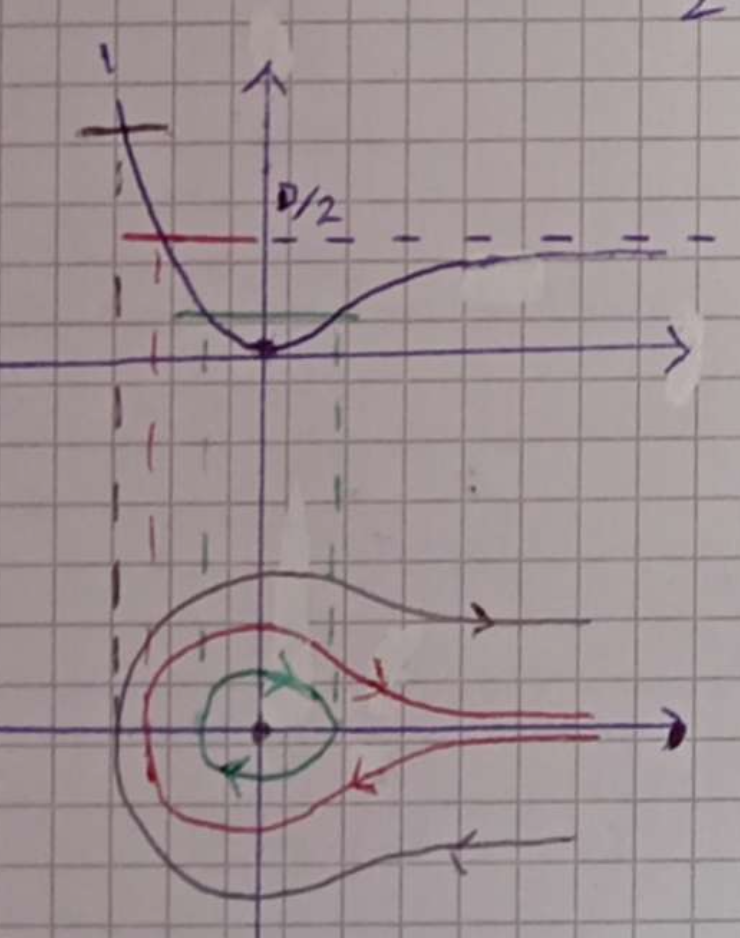
\includegraphics[width=0.6\textwidth]{images/potenzialeMorse.png}
    \caption{Ritratto in fase del potenziale di Morse}
\end{figure}

Studiamo il ritratto in fase del sistema:

\begin{itemize}
    \item $E < 0$: nessun moto
    \item $E = 0$: equilibrio $(0,0)$
    \item $0 < E < \tfrac{D}{2}$: moti periodici
    \item $E = \tfrac{D}{2}$: separatrice, moto illimitato
    \item $E > \tfrac{D}{2}$: moto illimitato con velocità asintotica:  $v_{\infty}^{\pm} = \pm \sqrt{\frac{2}{m}\left(E - \frac{D}{2}\right)}$
\end{itemize}


\subsubsection{Equazioni di Kortewieg de vries}

\begin{equation}
    \pdv{u}{t}= \pdv[3]{u}{x}+ u\pdv{u}{x} \qquad u(x,t),\;x \in \mathbb{R}
\end{equation}

Descrive il moto delle onde in \textit{fluidi ideali} a bassa profondità, viene studiata perché legata alle \textit{onde solitarie}, 
onde anomale in grado di propagarsi per chilometri nei canali arificiali. Descrive, inoltre, molto bene anche gli tsunami vicino alle coste.

Cerchiamo dunque soluzioni a onda:
\begin{equation}
    u(x,t) = f(x-ct), \quad c \in \mathbb{R}, \quad s = x - ct
\end{equation}
\begin{equation}
    \pdv{u}{t} = f'(s)\pdv{s}{t} = -c f'(s), 
    \qquad 
    \pdv{u}{x} = f'(s)\pdv{s}{x} = f'(s)
\end{equation}
\begin{equation}
    -c f'(s) = f'''(s) + f(s)f'(s)
    \implies 0 = \dv{s}\left( c f + f'' + \frac{f^2}{2} \right)
\end{equation}
\begin{equation}
    \implies f'' + c f + \frac{f^2}{2} = \text{costante} \equiv K
\end{equation}

Richiedendo che 
\[
u, \; \pdv{u}{x}, \; \pdv[2]{u}{x} \to 0 \quad \text{per } |x|\to\infty
\]
ossia che $f, f', f'' \to 0$ per $|s|\to\infty$, si ottiene $K =0$.

\begin{equation}
    \implies f'' = -c f - \frac{f^2}{2}
\end{equation}
è un'equazione di Newton per un punto di $m= 1$, di posizione $f $ al tempo $s $.
\begin{equation}
    U( f ) = \frac{cf^2}{2}+ \frac{f^3}{6} \qquad \frac{(f')^2}{2}+ U(f)= E 
\end{equation}

Consideriamo solo la soluzione omoclina per $c<0 $, dato che è l'unica ad avere senso fisico ($\lim_{s\rightarrow\infty}f=0$):

\begin{equation}
   \implies \frac{(f')^2}{2} + \frac{c}{2}f^2 + \frac{f^3}{6} = 0
\end{equation}
\begin{equation}
    f'_{\pm}(s) = \pm \sqrt{-c f^2(s) - \frac{f^3(s)}{3}}
\end{equation}


%esercizio

%esercizio scatola


\subsection{Equilibiri, stabilità, piccole oscillazioni}
Partiamo dai sistemi 1-dimensionali, che sono sempre risolvibili: $m\ddot{x} = - U'(x)$ con $x \in \mathbb{R}$.\\
Studiamo $x $ vicini a $\bar{x}$ tale che $U(\bar{x})=0, U''(\bar{x})>0$ cioè un minimo non degenere.
\begin{equation}
    x(t)= \bar{x}+ \xi(t)\implies m\ddot{\xi}= - U''(x)\xi + o(\xi)
\end{equation}
si ha dunque un moto quasi armonico.
Generalizziamo:
\begin{definition}
    Si dice \textit{sistema lagrangiano meccanico naturale} un sistema definito dalla lagrangiana:
    \begin{equation}
        \mathcal{L} = \frac{1}{2}\dot{q}\cdot A(q)\dot{q}- U (q)
    \end{equation}
\end{definition}
\begin{remark}
    $\mathcal{L}$ non dipende esplicitamente da $t$, dunque $H = K_2+ U$ si conserva.
\end{remark}
Inoltre:

\begin{equation}
    p = \pdv{\mathcal{L}}{\dot{q}} = A(q)\dot{q}
\end{equation}
\begin{equation}
    \dot{p}_i = \dv{t}\left( \sum_{s=1}^l A_{is}(q)\dot{q}_s \right)
    = \pdv{}{q_i}\left( \tfrac{1}{2}\sum_{s,k=1}^l A_{sk}(q)\dot{q}_s \dot{q}_k \right) - \pdv{U}{q_i}
\end{equation}
\begin{equation}
    \sum_{s=1}^l A_{is}(q)\ddot{q}_s
    + \sum_{s,k=1}^l \pdv{A_{is}(q)}{q_k}\dot{q}_s\dot{q}_k
    = \tfrac{1}{2}\sum_{s,k=1}^l \pdv{A_{sk}(q)}{q_i}\dot{q}_s\dot{q}_k - \pdv{U}{q_i}
\end{equation}
\begin{equation}
    (A(q)\ddot{q})_i = Q_i(q,\dot{q}) - \pdv{U}{q_i}
\end{equation}
\begin{equation}
    \ddot{q} = A^{-1}(q)\left[ Q(q,\dot{q}) - \pdv{U}{q} \right]
\end{equation}

Ponendo $v = \dot{q}$, il sistema diventa:
\begin{equation}
\begin{cases}
    \dot{q} = v \\
    \dot{v} = A^{-1}(q)\left[ Q(q,v) - \pdv{U}{q} \right]
\end{cases}
\end{equation}

Gli equilibri sono i punti per cui $\dot{q}=0, \; \dot{v}=0$, cioè:
\begin{equation}
    v=0, \qquad A^{-1}(q)\left[ Q(q,0) - \pdv{U}{q} \right] = 0
\end{equation}
\begin{equation}
    \iff v=0, \qquad \pdv{U}{q}=0
\end{equation}
Dunque gli equilibri stanno in punti $(\bar{q},0)$ con $\bar{q}$ punto critico di $U(q)$.


\begin{equation}
    q(t) = \bar{q} + \xi(t), \qquad v(t) = \dot{q}(t)
\end{equation}
\begin{equation}
\begin{cases}
    \dot{\xi} = v \\
    \dot{v} = A^{-1}(\bar{q}+\xi)\left[ Q(\bar{q}+\xi,v) - \pdv{U}{q} \left(\bar{q}+\xi\right) \right]
\end{cases}
\end{equation}

Sviluppando:
\begin{equation}
    \dot{v} = A^{-1}(\bar{q}+\xi)\left[ - \pdv[2]{U}{q}(\bar{q})\,\xi + o\big((\xi,v)\big) \right]
\end{equation}
\begin{equation}
    \dot{v} = A^{-1}(\bar{q})\left[ - \pdv[2]{U}{q}(\bar{q})\,\xi \right] + o\big((\xi,v)\big)
\end{equation}

\begin{equation}
    \implies \ddot{\xi} = - A^{-1}(\bar{q}) \pdv[2]{U}{q}(\bar{q})\,\xi
    \quad\iff\quad
    A(\bar{q})\ddot{\xi} = - \pdv[2]{U}{q}(\bar{q})\,\xi
\end{equation}

\begin{remark}
    \(\pdv[2]{U}{q}(\bar{q})\) è definita positiva (condizione di minimo stretto per \(U\)).
\end{remark}

Mostriamo che le equazioni lineari vengono dalla parte quadratica di L:

\begin{equation}
    L = \tfrac{1}{2}\dot{q}\cdot A(q)\dot{q} - U(q)
\end{equation}

Sviluppiamo intorno a $(\bar{q},0)$ con $q(t)=\bar{q}+\xi(t)$:
\begin{equation}
    L(\xi,\dot{\xi}) = \tfrac{1}{2}\dot{\xi}\cdot A(\bar{q}+\xi)\dot{\xi} - U(\bar{q}+\xi)
\end{equation}
\begin{equation}
    = \tfrac{1}{2}\dot{\xi}\cdot A(\bar{q})\dot{\xi} 
    - \pdv{U}{q}(\bar{q})\cdot \xi 
    - \tfrac{1}{2}\xi\cdot \pdv[2]{U}{q}(\bar{q})\,\xi
    + cost
    + o\left(\abs{(\xi,\dot{\xi})}^2\right)
\end{equation}

Poiché $\pdv{U}{q}(\bar{q})=0$, la lagrangiana quadraticizzata è:
\begin{equation}
    L_2(\xi,\dot{\xi}) = \tfrac{1}{2}\dot{\xi}\cdot A(\bar{q})\dot{\xi} 
    - \tfrac{1}{2}\xi\cdot \pdv[2]{U}{q}(\bar{q})\,\xi
\end{equation}

Dalle equazioni di Eulero-Lagrange:
\begin{equation}
    \dv{t}\left( \pdv{L_2}{\dot{\xi}} \right) = \pdv{L_2}{\xi}
    \iff
    A(\bar{q})\ddot{\xi} = - \pdv[2]{U}{q}(\bar{q})\,\xi
\end{equation}

Cerchiamo soluzioni del problema monodimensionale del tipo $\xi(t)=a\cos(\omega t)$. Allora:
\begin{equation}
    -m\omega^2 a\cos(\omega t) = -U''(\bar{x})\,a\cos(\omega t)
    \implies \omega = \sqrt{\tfrac{U''(\bar{x})}{m}}
\end{equation}

% ---- Problema agli autovalori generalizzato per le piccole oscillazioni ----
Poniamo
\begin{equation}
    A := A(\bar{q})\,, \qquad B := \pdv[2]{U}{q}\left(\bar{q}\right)
\end{equation}
con $A,B$ matrici simmetriche $L\times L$ e $A$ definita positiva. L'equazione linearizzata si scrive
\begin{equation}
    A\ddot{\xi} = - B\,\xi.
\end{equation}
Cerchiamo soluzioni del tipo
\begin{equation}
    \xi(t) = M\cos(\omega t), \qquad M\neq 0\quad M \in \mathbb{R}^L.
\end{equation}
Sostituendo otteniamo
\begin{equation}
    A(-\omega^2 M\cos(\omega t)) = - B M\cos(\omega t) \implies \omega^2 A M = B M,
\end{equation}
ossia il problema agli autovalori generalizzato
\begin{equation}
    (B - \omega^2 A) M = 0.
\end{equation}
Per una soluzione non banale vale
\begin{equation}
    \omega^2 = \frac{M\cdot (B M)}{M\cdot (A M)} \in \mathbb{R}, \qquad M\cdot (A M) > 0,
\end{equation}
perché $A$ è definita positiva e $B$ è simmetrica. Dunque $\omega$ è reale se $\omega^2>0$ oppure puramente immaginario se $\omega^2<0$.
Inoltre la condizione di esistenza è
\begin{equation}
    \det\big( B - \omega^2 A \big) = 0.
\end{equation}

Poiché $A$ è definita positiva, possiamo applicare il teorema spettrale: esistono autovalori positivi $\alpha_k>0$ e un sistema ortonormale di autovettori $\{w^{(k)}\}$ tali che
\begin{equation}
    A = \sum_{k=1}^L \alpha_k \, w^{(k)} \cdot (w^{(k)})^T.
\end{equation}
Definiamo allora la radice quadrata di $A$ come
\begin{equation}
    A^{1/2} = \sum_{k=1}^L \sqrt{\alpha_k} \, w^{(k)} \cdot (w^{(k)})^T,
\end{equation}
che verifica $(A^{1/2})^2 = A$. Analogamente si definisce $A^{-1/2}$.

La condizione di esistenza di soluzioni non banali
\begin{equation}
    \det(B - \omega^2 A) = 0
\end{equation}
è equivalente a
\begin{equation}
    \det(A^{-1/2} B A^{-1/2} - \omega^2 I) = 0.
\end{equation}
Quindi gli $\omega^2$ sono precisamente gli autovalori della matrice simmetrica
\begin{equation}
    C := A^{-1/2} B A^{-1/2},
\end{equation}

Definiamo
\begin{equation}
    \tilde{B} := A^{-1/2} B A^{-1/2}.
\end{equation}
Poiché $\tilde{B}$ è simmetrica, essa ammette una base ortonormale di autovettori $\{v^{(j)}\}_{j=1}^L \subset \mathbb{R}^L$ con autovalori reali $\omega_j^2$.  

Il problema agli autovalori
\begin{equation}
    (B - \omega^2 A)M = 0
\end{equation}
si traduce allora in
\begin{equation}
    (\tilde{B} - \omega^2 I)v = 0, 
    \qquad M = A^{-1/2} v.
\end{equation}

Dunque le soluzioni $M^{(j)}$ si ottengono dagli autovettori $v^{(j)}$ di $\tilde{B}$:
\begin{equation}
    M^{(j)} = A^{-1/2} v^{(j)}.
\end{equation}
Questi formano una base di $\mathbb{R}^L$ e risultano ortogonali rispetto al prodotto scalare definito da $A$:
\begin{equation}
    u^{(j)} \cdot A u^{(k)} = \delta^j_k, 
    \qquad u^{(j)} := A^{1/2} v^{(j)}.
\end{equation}

Concludiamo che il problema $(B - \omega^2 A)M=0$ ammette $L$ soluzioni indipendenti $(\omega_j^2, M^{(j)})$, con frequenze $\omega_j$ reali.

% Da sistemare questa parte


\begin{theorem}
    \textbf{Lagrange}  Esiste una trasformazione di coordinate $\xi\mapsto c $ tale che:
    \begin{equation}
        \mathcal{L}_2(c,\dot{c})= \sum_{j=1}^{L} \left( \frac{\dot{c}_j^2}{2}-\frac{w_j^2c_j^2}{2} \right)
    \end{equation}
    Le coordinate $c $ si dicono \textit{coordinate normali}.
\end{theorem}
\begin{proof}
    \begin{equation}
        \xi(t) = \sum_{j=1}^L c_j(t) M^{(j)}.
    \end{equation}

    Sostituendo nella lagrangiana quadratica otteniamo:
    \begin{equation*}
        \mathcal{L}_2(\xi,\dot{\xi}) 
        = \frac{1}{2} \left( \sum_{j=1}^L \dot{c}_j M^{(j)} \right) \cdot 
        A \left( \sum_{k=1}^L \dot{c}_k M^{(k)} \right) 
        - \frac{1}{2} \left( \sum_{j=1}^L c_j M^{(j)} \right) \cdot 
        B \left( \sum_{k=1}^L c_k M^{(k)} \right) 
    \end{equation*}
    \begin{equation}
        = \frac{1}{2} \sum_{j,k=1}^L \dot{c}_j \dot{c}_k \, (M^{(j)} \cdot A M^{(k)})
        - \frac{1}{2} \sum_{j,k=1}^L c_j c_k \, (M^{(j)} \cdot B M^{(k)}).
    \end{equation}

    Ora, usando le proprietà di ortogonalità e la relazione agli autovalori, segue:
    \begin{equation}
        M^{(j)} \cdot A M^{(k)} = \delta^j_k, 
        \qquad 
        M^{(j)} \cdot B M^{(k)} = \omega_j^2 \delta^j_k.
    \end{equation}

    La lagrangiana si diagonalizza quindi come
    \begin{equation}
        \mathcal{L}_2(\xi,\dot{\xi}) 
        = \sum_{j=1}^L \left( \frac{\dot{c}_j^2}{2} - \frac{\omega_j^2}{2} c_j^2 \right).
    \end{equation}
\end{proof}


\begin{definition}
    I moti indipendenti $c_j(t)M^{(j)}$ si chiamano \textit{modi normali di oscillazione} se $\omega_j^2>0$.
\end{definition}
\begin{definition}
    La mappa $\xi\mapsto c $ che diagonalizza $\mathcal{L}_2$ si chiama \textit{riduzione ai modi normali}.
\end{definition}
\begin{definition}
    Nel caso $\omega^2>0$, le $\omega$ si dicono \textit{frequenze caratteristiche} o \textit{proprie} o \textit{normali} e i vettori $M^{(j)}$ 
    si dicono \textit{vettori caratteristici} o ... 
\end{definition}

\begin{remark}
    \begin{equation}
        \dv{t}\pdv{\mathcal{L}_2}{\dot{c}_j}= \pdv{\mathcal{L}_2}{c_j}\iff \ddot{c}_j= - \omega_j^2c_j
    \end{equation}
    \begin{equation}
    \begin{cases}
        \omega_j^2 > 0 
        &\implies \; 
        c_j(t) = \alpha_j \cos(\omega_j t) + \beta_j \sin(\omega_j t), \\[6pt]
        \omega_j^2 < 0 
        &\implies \; 
        c_j(t) = \gamma_j e^{\sqrt{-\omega_j^2}\,t} + \delta_j e^{-\sqrt{-\omega_j^2}\,t}.
    \end{cases}
    \end{equation}
\end{remark}



\subsection{Stabilità secondo Lyapunov}

Consideriamo un sistema di equazioni differenziali ordinarie in $\mathbb{R}^n$
\begin{equation}
    \dot{x} = u(x), \quad x \in \mathbb{R}^n, \quad u : \mathbb{R}^n \to \mathbb{R}^n, \quad u \in \mathcal{C}^k, \; k \geq 1
\end{equation}

cioè, in forma esplicita
\begin{equation*}
    \begin{cases}
        \dot{x}_1 = u_1(x_1, \dots, x_n) \\
        \quad \vdots \\
        \dot{x}_n = u_n(x_1, \dots, x_n).
    \end{cases}
\end{equation*}

La soluzione del sistema
\begin{equation}
    \begin{cases}
        \dot{x} = u(x) \\
        x(0) = x_0
    \end{cases}
\end{equation}
è detta \textit{flusso} e si indica con
\begin{equation}
    x(t) \equiv \Phi^t(x_0),
\end{equation}
associato al campo vettoriale $u$.

Un punto $\bar{x}$ tale che
\begin{equation}
    u(\bar{x}) = 0
\end{equation}
si dice \textit{punto di equilibrio} del sistema.

In tal caso
\begin{equation}
    x(t) = \bar{x}, \quad \forall t
\end{equation}
è soluzione, cioè
\begin{equation}
    \Phi^t(\bar{x}) = \bar{x}, \quad \forall t.
\end{equation}

Supponiamo ora che $\bar{x}$ sia isolato e sfruttiamo l’equivalenza delle norme in $\mathbb{R}^n$.

\begin{definition}
Il punto di equilibrio $\bar{x}$ si dice \textit{stabile} se $\forall \, J$ intorno di $\bar{x}$, 
$\exists \, I$ intorno di $\bar{x}$, con $I \subseteq J$, tale che
\[
x_0 \in I \implies \varphi^t(x_0) \in J, \quad \forall t \geq 0.
\]
\end{definition}

\begin{definition}
$\bar{x}$ è \textit{asintoticamente stabile} se è stabile e 
\[
\lim_{t \to +\infty} \varphi^t(x_0) = \bar{x}, \quad \forall x_0.
\]
\end{definition}

\begin{remark}
Soltanto per $J = B_\varepsilon(\bar{x})$, $I = B_{\delta(\varepsilon)}(\bar{x})$ 
\[
(\forall \varepsilon > 0, \, \exists \, \delta(\varepsilon) > 0, \, \delta(\varepsilon) \leq \varepsilon \, : \, 
\forall x_0 \in B_{\delta(\varepsilon)}(\bar{x}), \, \varphi^t(x_0) \in B_\varepsilon(\bar{x}) \,\, \forall t \geq 0).
\]
\end{remark}
\begin{definition}
    Un punto di equilibrio si dice \textit{instabile} se non è stabile.
\end{definition}
\begin{example}
    I punti elittici sono stabili, i punti iperbolici sono instabili.
\end{example}

\begin{definition}
    Si dice \textit{funzione di Lyapunov}, la funzione $W: \mathbb{R}^n\mapsto \mathbb{R}$, data per $u(x)= \dot{x}$, tale che:
    \begin{itemize}
        \item[(i)]$W(x)$ ha minimo locale stretto in $\bar{x}$, con $W(\bar{x})=0, \ W(x)>0 \;\;\forall\, x \in K\backslash\{\bar{x}\}$
        \item[(ii)] $L_uW(x):=u(x)\cdot\nabla W(x)\leq 0 \;\;\forall\,x \in K$
    \end{itemize} 
    $L_uW$ si dice \textit{derivata direzionale} o di Lie di $W$ lungo il campo vettoriale $u$.
\end{definition}
\begin{remark}
    \begin{equation}
        \dv{t}W(x(t))= \sum_{j=1}^{n }\pdv{W}{x_j}\cdot\dot{x}_j= \sum_{j=1}^{n}u_j(x)\pdv{W}{x_j}= u(x)\cdot \nabla W(x)= L_uW(x)
    \end{equation}
\end{remark}


\begin{theorem}
    \textbf{Lyapunov}\\
    Se esiste funzione locale $W(x)$ per $\bar{x}$ allora $ \bar{x}$ è stabile,
    se inoltre $L_uW(x)<0\ \forall\,x$ allora è asintoticamente stabile.
\end{theorem}
\begin{proof}
Sia $J < K$, e sia $\alpha = \min_{\partial J} W(x) > 0$ (per Weierstrass).  

Definiamo
\begin{equation*}
    G_\alpha \equiv \{ x \in J \mid W(x) < \alpha \}, \quad G_\alpha \subseteq J
\end{equation*}

Osserviamo che $\bar{x} \in G_\alpha$ perché $W(\bar{x}) = 0 < \alpha$.  

La funzione $\alpha - W(x)$ è positiva in $\bar{x}$ e, essendo continua, esiste un intorno di $\bar{x}$ tale che
\begin{equation*}
    \alpha - W(x) > 0, \quad \forall x \in J
\end{equation*}

Per ipotesi (ii),
\begin{equation*}
    \dv{t} W(x(t)) \leq 0 \quad (= L_u W(x(t))).
\end{equation*}
\begin{equation*}
   \implies W(x(t)) \leq W(x(0)) \implies x(0) \in G_\alpha \implies x(t) \in G_\alpha, \ \forall t.
\end{equation*}

Dunque $G_\alpha \subset J \implies x(t) \in J, \ \forall t$.  

Per il secondo punto:  
\begin{equation*}
    \dv{t} W \leq 0 \quad \implies \quad W(x(t)) \ \text{monotona decrescente nel tempo}.
\end{equation*}

Se la decrescita è stretta, allora $W(x(t))$ è monotona decrescente strettamente, inferiore limitata e per assurdo è possibile dimostrare che
\begin{equation*}
    \lim_{t \to +\infty} W(x(t)) = \inf W = 0
\end{equation*}
\end{proof}


\begin{example}
    \textbf{Oscillatore armonico smorzato.}\\
    \begin{equation}
        m\ddot{x} = -kx - \gamma \dot{x}
        \implies 
        \begin{cases}
            \dot{x} = v \\
            \dot{v} = -\dfrac{k}{m}x - \dfrac{\gamma}{m} v
        \end{cases}
    \end{equation}

    \begin{equation}
        H(x,v) = \frac{m}{2}v^2 + \frac{k}{2}x^2 \quad \text{soddisfa (i)}
    \end{equation}

    \begin{equation}
        \dv{H}{t} = kx\dot{x} + mv\dot{v} 
        = kxv + mv\left(-\frac{k}{m}x - \frac{\gamma}{m} v \right) 
        = - \gamma v^2 \leq 0
    \end{equation}
\begin{remark}
    \begin{equation*}
         L_v H = 
        \left(v,\; -\frac{k}{m}x - \frac{\gamma}{m} v \right) 
        \cdot \left(kx,\; mv \right) 
        = - \gamma v^2
    \end{equation*}
\end{remark}

\end{example}


\begin{theorem}
    \textbf{Dirichlet- Lagrange}\\
    Dato un sistema meccanico naturale con 
    \begin{equation}
        \mathcal{L}(q,\dot{q})=\frac{1}{2}\dot{q}\cdot A(q)\dot{q} - U(q)
    \end{equation}
    se $\bar{q}$ è minimo locale stretto per $U(q)$, allora $(\bar{q},0) \in \mathbb{R}^{2L}$ è stabile secondo Lyapunov.
\end{theorem}
\begin{proof}

\begin{equation}
    H(q,\dot{q}) = \tfrac{1}{2} \dot{q}\cdot A(q)\dot{q} + U(q) \quad \text{ si conserva.}
\end{equation}
  

Definiamo
\begin{equation}
    W(q,\dot{q}) = H(q,\dot{q}) - U(\bar{q}),
\end{equation}
che è una funzione di Lyapunov locale.  

\begin{itemize}
    \item[(i)] $W(\bar{q},0) = H(\bar{q},0) - U(\bar{q}) = 0$.  
    Inoltre  $
        W(q,\dot{q}) = \tfrac{1}{2}\dot{q}\cdot A(q)\dot{q} + U(q) - U(\bar{q}) > 0
    $
    in un intorno di $(\bar{q},0)$.  

    \item[(ii)] $L_u W = 0$, poiché $\dot{W} = \dot{H} = 0$ lungo le soluzioni delle equazioni di Lagrange.  
\end{itemize}

Dunque si applica il teorema di Lyapunov.  

\end{proof}

\begin{remark}
    Se si aggiunge una forza di attrito viscoso $-\gamma v$, il punto diventa asintoticamente stabile.
\end{remark}
\begin{remark}
    Nel caso conservativo, $(\bar{q},0)$ non può essere asintoticamente stabile.
\end{remark}
\begin{proof}
    $\lim_{t\rightarrow\infty}(q,\dot{q})= (\bar{q},0)$ implica che $\lim_{t\rightarrow\infty}H(q,\dot{q})= H(\bar{q},0)= U(\bar{q})$ 
    il che è assurdo perché $H(q,\dot{q})\equiv E >U(\bar{q})$
\end{proof}

\begin{proposition}
Sia $\bar{q}$ un minimo locale non degenere di $U$, cioè $B:=\pdv[2]{U}{q}(\bar{q})>0$. Allora, ponendo $\xi:=q-\bar{q}$, vicino a $(\bar{q},0)$ vale
\begin{equation}
    W(q,v)=\frac{1}{2}\,v\cdot A(\bar{q})\,v+\frac{1}{2}\,\xi\cdot B\,\xi+o\!\left(\norm{(\xi,v)}^2\right).
\end{equation}
Definendo
\begin{equation}
    \xi'=A^{1/2}\xi \qquad\text{e}\qquad \tilde{B}:=A^{-1/2}BA^{-1/2},
\end{equation}
si ha
\begin{equation}
    W=\frac{1}{2}\,\abs{v'}^2+\frac{1}{2}\,\xi'\cdot \tilde{B}\,\xi'+o\!\left(\norm{(\xi',v')}^2\right).
\end{equation}
Poiché $\tilde{B}$ è simmetrica definita positiva, esiste $R\in O(L)$ tale che
\begin{equation}
    R^\intercal \tilde{B} R=D=\operatorname{diag}(\omega_1^2,\dots,\omega_L^2),\ \ \omega_j^2>0.
\end{equation}
Ponendo
\begin{equation}
    \xi'=R\,\xi'' \qquad v''=R\,v'
\end{equation}
segue
\begin{equation}
    W=\frac{1}{2}\,\abs{v''}^2+\frac{1}{2}\sum_{j=1}^{L}\omega_j^2\,(\xi''_j)^2+o\!\left(\norm{(\xi'',v'')}^2\right)\equiv E'
\end{equation}
cioè, a primo ordine non banale, i livelli di $W$ sono ellissoidi e il sistema è somma di oscillatori indipendenti con frequenze $\omega_j$.
Dividendo per $E>0$:
\begin{equation}
    \sum_{j=1}^{L}\left( \frac{(\xi''_j)^2}{\tfrac{2E}{\omega_j^2}} + \frac{(v''_j)^2}{2E} \right)=1,
\end{equation}
che rappresenta un’ellisse in ciascun piano $(\xi''_j,v''_j)$.


Dunque se $\bar{q}$ è punto critico non degenere, con $B=\pdv[2]{U}{q}(\bar{q})$, allora
\begin{itemize}
    \item se $B>0$, $(\bar{q},0)$ è $L$-stabile;
    \item se $B<0$ (alcuni $\omega_j^2<0$), $(\bar{q},0)$ è instabile con oscillazioni iperboliche;
    \item se $B$ è indefinita, $(\bar{q},0)$ è instabile.
\end{itemize}

\end{proposition}